\documentclass[a4paper, notitlepage, 9pt]{extreport}
\usepackage[italian]{babel}
\usepackage[T1]{fontenc}
\usepackage[utf8]{inputenc}
\usepackage{amsmath}
\usepackage{amsfonts}
\usepackage{amsthm}
\usepackage{frontespizio}
\usepackage{hyperref}
\hypersetup{hidelinks,
	colorlinks = true,
	urlcolor = black, 
	linkcolor = black}
\usepackage[margin=3cm]{geometry}
\usepackage{booktabs}
\usepackage{fancyhdr}
\usepackage{listings}
\setcounter{tocdepth}{4}
\usepackage{stmaryrd}
\usepackage[strict]{changepage}
\usepackage{libertine}
\usepackage{textcomp}
\usepackage{float}
\usepackage{multicol}
\usepackage{makecell}
\usepackage{stmaryrd}
\usepackage{amssymb}
\usepackage{caption}
\renewcommand\theadalign{bc}
\renewcommand\theadfont{\bfseries}
\renewcommand\theadgape{\Gape[4pt]}
\renewcommand\cellgape{\Gape[4pt]}

\lstset{basicstyle=\ttfamily\small}

\makeatletter
\newcommand*{\toccontents}{\@starttoc{toc}}
\makeatother

\begin{document}
	\title{\textbf{\underline{Sistemi Informativi}}}
	\date{Febbraio - Marzo 2018}
	\author{Colognese, Rossini}
	\maketitle
	
	\toccontents

\chapter*{Teoria dell'Organizzazione}
\addcontentsline{toc}{chapter}{Teoria dell'Organizzazione}
Il \textit{\textbf{Sistema Informativo}} è la componente di una \textit{organizzazione} (persone e tecnologie) che \textit{gestisce} (analizza, elabora, estrapola) le \textit{informazioni di interesse} (utilizzate e prodotte durante l'esecuzione dei processi).

\section*{Organizzazione Aziendale}
\addcontentsline{toc}{section}{Organizzazione Aziendale}
L'\textit{\textbf{Organizzazione}} è il processo attraverso il quale un insieme di persone viene strutturato secondo i principi di divisione del lavoro e coordinamento, diventando un sistema (sinonimo di azienda).

Un'azienda è un'organizzazione di persone e tecnologie finalizzata alla soddisfazione di bisogni umani attraverso la produzione, la distribuzione o il consumo di beni economici.
\begin{itemize}
	\item Dall'interazione tra risorse umane e tecnologie deriva il \textit{\textbf{comportamento aziendale}}, rivolto al raggiungimento degli obiettivi, che produce dei risultati.
\end{itemize}

\noindent
L'\textit{\textbf{Organizzazione Aziendale}} è il processo attraverso il quale l'insieme di persone che partecipano direttamente allo svolgimento delle attività dell'azienda viene strutturato secondo i principi di divisione del lavoro e coordinamento (ruoli e funzioni diverse, seguendo scopi, metodi e regole). Contiene dei macroprocessi (operativo/produttivo, controllo e gestione) e dispone di risorse (umane, materiali, \textit{informative}).

\noindent
\textit{\textbf{Teoria dell'Organizzazione}}: studio e progettazione scientifica dei compiti per
migliorare le prestazioni.

\section*{Tecnologie Informatiche}
\addcontentsline{toc}{section}{Tecnologie Informatiche}
Le \textit{\textbf{Tecnologie Informatiche}} sono un insieme di sistemi, strumenti e tecniche per automatizzare il trattamento delle informazioni. Portano innovazione scientifica e tecnica, riduzione dei tempi e costi di produzione. Supportano il ciclo di vita dell’informazione come risorsa aziendale (è oggetto di processi produttivi, operativi e attività gestionali).

\noindent
Le \textit{\textbf{Infrastrutture di Tecnologie Informatiche}} sono un insieme di risorse tecnologiche condivise che fornisce una piattaforma per le applicazioni informatiche di un’azienda. Include investimenti in hardware, software e servizi (consulenze, aggiornamenti e training del personale).

\noindent
Un \textit{\textbf{Sistema Informativo Aziendale}} è un insieme di elementi interconnessi che raccolgono, catalogano, ricercano, elaborano, memorizzano e distribuiscono dati trasformandoli in informazioni utili per supportare le attività decisionali di controllo di un’azienda.

Deve essere progettato per svolgere tre macroprocessi: acquisizione dei dati (processo di Input), trasformazione dei dati (processo di Elaborazione) e restituzione di informazioni (processo di Output).

I \textit{sistemi informativi} svolgono la funzione di automatizzare la gestione e l’elaborazione dei dati.

\begin{multicols}{2}
	\begin{figure}[H]
		\centering
		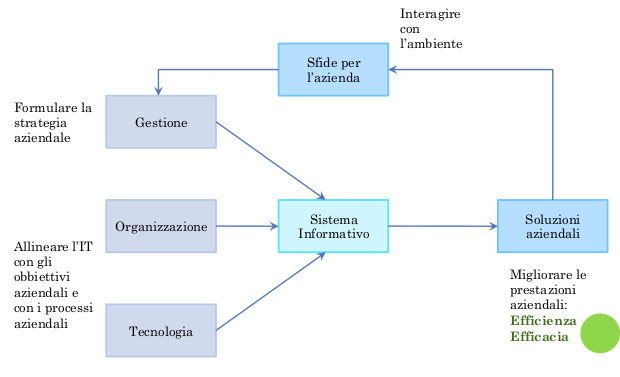
\includegraphics[height=4.5cm]{SistemaInformativoAziendale}
	\end{figure}
	\columnbreak
	\noindent
	Il \textit{sistema produttivo} si basa su: obiettivi (output atteso), input e output (effettivo).

	\begin{itemize}
		\item \textit{Efficienza}: costo per il raggiungimento degli obiettivi.
		\item \textit{Efficacia}: grado di raggiungimento degli obiettivi.
	\end{itemize}
	\begin{figure}[H]
		\centering
		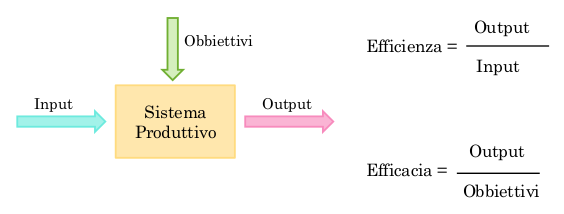
\includegraphics[scale=0.32]{EfficienzaEfficacia}
	\end{figure}
\end{multicols}

Le \textit{tecnologie informatiche} hanno un impatto positivo sull'\textit{\textbf{efficienza}} dei sistemi produttivi: riducono i costi unitari, aumentano la produzione a parità di risorse (aspetto quantitativo), incentiva la crescita delle dimensioni organizzative e cambia la struttura organizzativa.
\newline

Le \textit{tecnologie informatiche} hanno aumentano l'\textit{\textbf{efficacia}} dei sistemi produttivi: uso più efficiente dei fattori produttivi a parità di volumi di produzione, razionalizzazione dell'uso delle risorse (aspetto qualitativo), differenziazione dei prodotti e ampliamento della gamma.
\newline

A livello operativo le \textit{tecnologie informatiche} hanno semplificato i compiti individuali, dato una maggiore specializzazione, aumentato l'interdipendenza e incrementato la complessità gestionale.

\section*{Gestione dell'Informazione}
\addcontentsline{toc}{section}{Gestione dell'Informazione}
La \textit{gestione dell’informazione} è quindi fondamentale per il raggiungimento degli scopi aziendali:
\begin{itemize}
	\item \textit{\textbf{informazione}} come \textit{\textbf{risorsa organizzativa}} fondamentale.
\end{itemize}
\noindent
L'\textit{\textbf{informazione}} è la risorsa principale: viene scambiata, selezionata ed elaborata nelle attività gestionali di controllo e coordinamento.

Viene prodotta da qualunque attività (anche operativa) ma è una \textit{risorsa immateriale} che sta alla base di ogni altra risorsa immateriale (conoscenza ed esperienza individuale ed organizzativa). Non viene distrutta dall'uso, può essere soggetta ad obsolescenza, non si esaurisce ma \textit{si auto-rigenera} (cioè estraggo un'informazione e da essa ne posso dedurre altre, incrementando le prestazioni dei processi gestionali).
\newline

\noindent
La quantità di informazione posseduta può causare:
\begin{itemize}
	\item \textit{Overload informativo}: aumento incontrollato dell'informazione disponibile, eccedendo le capacità di elaborazione individuale; causando rallentamento e peggioramento delle decisioni.
	\item \textit{Underload informativo}: disponibilità di informazioni al di sotto delle capacità di elaborazione individuale; semplificazione delle decisioni che vengono prese in tempi più brevi.
\end{itemize}

\section*{Organizzazione come Sistema Aperto}
\addcontentsline{toc}{section}{Organizzazione come Sistema Aperto}
In funzione delle opportunità fornite dall’\textit{ambiente
esterno} e tenendo conto dei vincoli da esso posti, l’azienda definisce i propri obiettivi.

Deve inoltre sapersi adattare ai cambiamenti dell'ambiente esterno (nuovi requisiti come ad esempio un cambio di mode), dunque all'\textbf{\textit{incertezza ambientale}}. Esiste un \textit{\textbf{cruscotto aziendale}} che prende decisioni strategiche in base ai dati che arrivano dall'esterno.
\newline

\noindent
L'\textit{informazione} gioca un ruolo fondamentale nel determinare la capacità di adattamento come risorsa delle attività gestionali di ripianificazione organizzativa.
\newline

\noindent
\textit{\textbf{Capacità elaborativa}}: adeguatezza di un’organizzazione rispetto alle necessità di elaborare informazioni a essa imposte dai propri obiettivi e dal contesto in cui opera.

\subsection*{Modello Gerarchico (Piramide di Anthony)}
\addcontentsline{toc}{subsection}{Modello Gerarchico (Piramide di Anthony)}
\begin{multicols}{2}
	\begin{figure}[H]
		\centering
		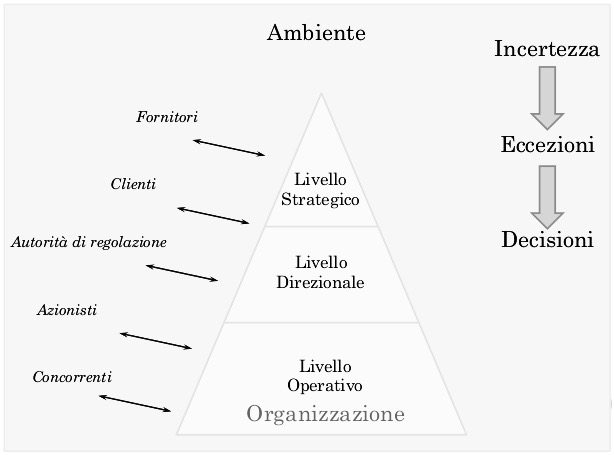
\includegraphics[scale=0.40]{Piramide1}
	\end{figure}
	\columnbreak
	\begin{figure}[H]
		\centering
		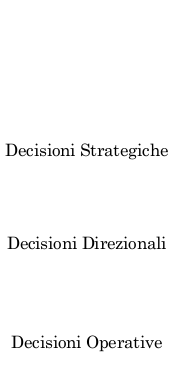
\includegraphics[scale=0.45]{Piramide2}
	\end{figure}
\end{multicols}
\begin{itemize}
	\item I cambiamenti delle tendenze di mercato comportano una ripianificazione strategica degli obiettivi di produzione.
	\item Un malfunzionamento HW può essere gestito al livello di competenza senza far salire l'informazione al livello più alto (\textit{\small{se servono matite non si mandano richieste al livello strategico}}).
\end{itemize}

\noindent
La capacità elaborativa di un'organizzazione dovrebbe essere superiore a quella di ciascuno degli individui che la compongono. L'organizzazione supera i limiti individuali.

\subsection*{Progettazione del Sistema Informativo}
\addcontentsline{toc}{subsection}{Progettazione del Sistema Informativo}
La progettazione del Sistema Informativo è un’attività fortemente legata alla pianificazione della struttura organizzativa. Il Sistema Informativo massimizza le prestazioni dell’organizzazione.

\noindent
\textit{\textbf{Allineamento fra Sistema Informativo, struttura organizzativa e livello di incertezza}}: Come organizzare gli scambi informativi all’interno di una organizzazione a fronte di crescente incertezza ambientale.
\begin{figure}[H]
	\centering
	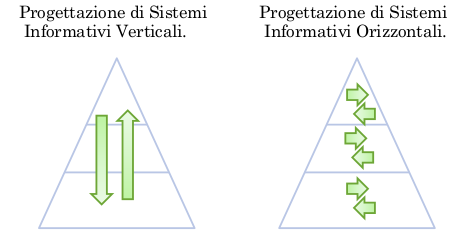
\includegraphics[scale=0.40]{SIVertOriz}
\end{figure}

\noindent
\textit{\textbf{Sistemi Informativi Verticali}}: storicamente i primi ad essere supportati da sistemi informatici. Accentramento delle decisioni. Al crescere dell’incertezza e del numero di eccezioni, i livelli gerarchici superiori vengono sovraccaricati dai compiti decisionali.

Limite: capacità elaborativa dell’organizzazione coincide con la capacità elaborativa dell’unità gerarchicamente più elevata (che potrebbe essere un individuo).
\newline

\noindent
\textit{\textbf{Sistemi Informativi Orizzontali}}: comunicazione fra unità organizzative allo stesso livello, anche se dipendenti gerarchicamente da unità distinte. Delega decisionale.

\noindent
Collegamenti laterali a crescente capacità elaborativa:
\begin{itemize}
	\item contatti diretti tra coloro che condividono lo stesso problema;
	\item gruppi temporanei di lavoro (task force) o permanenti (team);
	\item ruoli manageriali di integrazione per gestire le eccezioni relative ad un particolare prodotto (\textit{\small{productmanager}}), programma (\textit{\small{program manager}}) o progetto (\textit{\small{project manager}});
	\item organizzazione a matrice, dunque ciascuna unità ha una doppia dipendenza gerarchica secondo due dimensioni rilevanti ai fini organizzativi(\textit{\small{ad esempio il docente sotto facoltà e dipartimento}}).
\end{itemize}

\subsection*{Inceretezza Comportamentale}
\addcontentsline{toc}{subsection}{Inceretezza Comportamentale}
Non esiste soltanto l’incertezza ambientale, ma anche l’incertezza legata ad un comportamento non prevedibile degli individui (\textit{\small{ad esempio un lavoratore che si sveglia male e rende di meno}}).

Si deve considerare l’eventualità che un individuo
decida di non scegliere la soluzione che massimizza l’efficienza e l’efficacia organizzativa (\small{trattenendo/nascondendo informazione invece di scambiarla, non rilevando eccezioni o non eseguendo il proprio compito decisionale}).

Si deve tener conto che gli individui sono mossi anche da interessi personali (spesso in conflitto con quelli organizzativi) e da comportamento opportunistico.
Queste divergenze rendono necessarie delle forme di coordinamento che generano dei costi di controllo (per la verifica del comportamento) e di garanzia (produzione documentata). Diventa dunque necessario attuare una \textit{minimizzazione dei costi} di produzione e coordinamento.



\chapter*{Classificazione dei Sistemi Informativi}
\addcontentsline{toc}{chapter}{Classificazione dei Sistemi Informativi}
Disposizione dei \textit{Sistemi Informativi} lungo la piramide aziendale (definizione e funzioni attribuite dipendono dal livello al quale essi sono collocati):
\begin{itemize}
	\item \textit{\textbf{Transaction Processing Systems (TPS)}}: alla base della piramide, destinati alla gestione delle transazioni, tengono traccia delle informazioni di routine nelle organizzazioni (ordini, spedizioni, ecc.);
	\item \textit{\textbf{Management Information Systems (MIS)}}: al livello superiore, destinato al management; acquisiscono dati dai TPS per fare una rappresentazione periodica della situazione delle operazioni aziendali;
	\item \textit{\textbf{Decision Support Systems (DSS)}}: allo stesso livello dei precedenti, affiancano il management nelle decisioni di non-routine per il supporto nelle decisioni aziendali; permettono di simulare ipotesi per testare la validità di una gestione, utilizzando i dati dai TPS e MIS e aggiungendo dati provenienti da fonti esterne (prezzi materie prime, tassi di mercato, ecc.);
	\item \textit{\textbf{Executive Information Systems (EES)}}: al vertice della gerarchia, sono riservati al senior manager dell'organizzazione per le decisioni strategiche di non-routine; sono spesso composti nel formato di un \textit{cruscotto digitale} con il quale il senior manager riesce ad avere sotto controllo gli andamenti della gestione aggregando informazioni interne ed esterne, sintetizzandole con gli indicatori più importanti.
\end{itemize}

\section*{Segmentazione dei Bisogni: il Portafoglio Applicativo}
\addcontentsline{toc}{section}{Segmentazione dei Bisogni: il Portafoglio Applicativo}
Il \textit{\textbf{Portafoglio Applicativo}} è l'insieme delle applicazioni utili in azienda e può essere diviso in tre segmenti principali:
\begin{itemize}
	\item \textit{\textbf{Portafoglio Direzionale}}: comprende le applicazioni informatiche a supporto dei cicli di pianificazione e controllo strategico e di pianificazione e controllo delle risorse aziendali (controllo budget, reporting, ecc.).
	
	\item \textit{\textbf{Portafoglio Istituzionale}}: comprende le applicazioni informatiche per i processi di supporto all’amministrazione, alla gestione delle risorse umane alla contabilità:
	\begin{itemize}
		\item processi che eseguono adempimenti di legge (contabilità, retribuzione, previdenza);
		\item processi che supportano l'amministrazione di infrastrutture (immobili);
		\item processi che supportano l’amministrazione di fattori di produzione (personale, scorte, denaro, impianti).
	\end{itemize}
	Riguarda aree con elevante potenzialità di informatizzazione (forte proceduralità, ripetitività, periodicità).
	
	L'informatizzazione nel portafoglio istituzionale inizia negli anni 90 con i sistemi \textit{ERP (Enterprise Resource Planning)} riducendo i costi di elaborazione (aumentandone la capacità) e rendendo più efficaci i processi di pianificazione, controllo e ottimizzazione.
	
	\item \textit{\textbf{Portafoglio Operativo}}: comprende le applicazioni informatiche per i processi primari della \textit{Catena del Valore di Porter} (acquisizione materie prime, fabbricazione, marketing, vendita, distribuzione, post-vendita).
	
	L'informatizzazione del portafoglio operativo porta i seguenti benefici:
	\begin{itemize}
		\item aumento della complessità gestibile nei processi aziendali;
		\item sincronizzazione dei dati all’interno dell’impresa (basi di dati uniche).
	\end{itemize}
\end{itemize}

\noindent
I portafogli \textit{direzionale} e \textit{istituzionale} due sono \textit{orizzontali}: generali, per tutti i settori. Indipendenti dalle specifiche caratteristiche dei settori. Il portafoglio \textit{operativo} è \textit{verticale}: specifico di ciascun settore industrale poiché l'attrattiva informatica dei settori è variabile (molto alta nel settore bancario).

\subsection*{Informatizzazione del Portafoglio Operativo nelle Imprese Manifatturiere}
\addcontentsline{toc}{subsection}{Informatizzazione del Portafoglio Operativo nelle Imprese Manifatturiere}
\textit{1960-1990: Procedure per automazione di singole attività} con soluzioni ad-hoc, linguaggi di programmazione classici (COBOL, C++) per migliorare l'efficienza nell'elaborazione dei dati e ottimizzare le risorse (meno scorte in magazzino).

\noindent
\textit{Dal 1970 al 1995: Pacchetti MRP (Manufacturing Resource Planning)}. \textit{MRP} è una tecnica che calcola i fabbisogni dei materiali e pianifica gli ordini di produzione e di acquisto, tenendo conto della domanda del mercato, della distinta base (materie prime per realizzare il prodotto), dei \textit{lead time} di produzione e di acquisto e delle giacenze dei magazzini.

I \textit{pacchetti MRP} erano inizialmente finalizzati alla sola informatizzazione del fabbisogno delle materie prime, produzione e gestione dei materiali (poi estesi a tutta la produzione). Fra le tecnologie chiave troviamo i database e pacchetti integrati. Tra i benefici troviamo: integrazione orizzontale e verticale dei processi intra-organizzativi e il bilanciamento dei fattori produttivi ed efficienza del processo di produzione.
\newline

\noindent
\textit{Dal 1980: CIM (Computer Integrated Manufacturing) - Automazione di fabbrica} con la gestione di parti di produzione affidate all’automazione computerizzata. Si ottiene l'eliminazione dei tempi morti e l'efficienza del processo di fabbricazione e qualità dei prodotti.
\newline

\noindent
\textit{Dal 1990: Pacchetti ERP (Enterprise Resource Planning)} con gestione produzione, integrata con applicazioni a supporto dei processi di vendita e distribuzione fisica (controllo degli inventari, tracciamento degli ordini, servizi per i clienti, finanza e risorse umane). Le tecnologie chiave sono le architetture client-server e la rete (1997/98). I benefici sono rappresentati dalla trasformazione dei processi interni all’azienda e una maggiore efficienza dei fattori produttivi.
\newline

\noindent
\textit{Dal 1995: Sistemi CRM (Customer Relationship Management)} (per la fidelizzazione del cliente) con gestione della distribuzione, vendita e post-vendita. Le tecnologie chiave sono i pacchetti integrati per l’intero ciclo sul cliente e le architetture client-server e Web. I benefici sono rappresentati dall'abbattimento dei costi di transazione per il cliente e l'integrazione orizzontale e verticale dei processi di gestione dei clienti.
\newline

\noindent
\textit{Dal 1995: E-Procurement} con l'informatizzazione del buy-side delle imprese utilizzando pacchetti per l’intero ciclo di acquisto e architetture basate su tecnologie Internet(acquisizione di beni e servizi attraverso la rete). I benefici sono l'abbattimento dei costi di transazione per il compratore e per il venditore e l'integrazione orizzontale e verticale dei processi di gestione dei fornitori.


\section*{Enterprise Resource Planning (ERP)}
\addcontentsline{toc}{section}{Enterprise Resource Planning (ERP)}
\textit{ERP} indica una suite di moduli applicativi che supportano l’intera gamma dei processi di un’azienda.

\noindent
Evoluzione dello schema \textit{MRP} esteso ad attività amministrative e finanziarie, vendita e post-vendita, attività gestionali.

\noindent
Con la seguente architettura troviamo:
\begin{itemize}
	\item sistemi modulari composti da \textit{database server} (gestione dati), \textit{application server} (elaborazione dati), \textit{presentation server} (presentazione dati);
	\item una base di dati condivisa per sincronizzare i processi interdipendenti, minimizzare i dati da immettere e garantire la coerenza delle informazioni.
\end{itemize}
Questi sistemi interagiscono tramite interfacce (con possibilità di estenderli), sono configurabili, serve periodo di avviamento (costoso e induce a ridefinizione dei processi aziendali) ed è presente sul mercato in modalità standard pre-configurata (inducono all'omologazione). Sono molto diffusi poiché i moduli sono venduti separatamente e parametrizzabili in base all'azienda che li usa.

Questi sistemi accelerano i cicli operativi e la condivisione dell'operazione (abbattendo i costi delle transazioni), però obbligano l’azienda ad adattare le procedure gestionali al sistema.

\MakeUppercase{è} applicabile a diversi settori mediante: la presenza di moduli indipendenti che coprono una specifica area aziendale, la struttura globale \textit{ERP} unica in cui cambiano i moduli di gestione del \textit{core-business} aziendale.
\begin{multicols}{2}
	\begin{figure}[H]
		\centering
		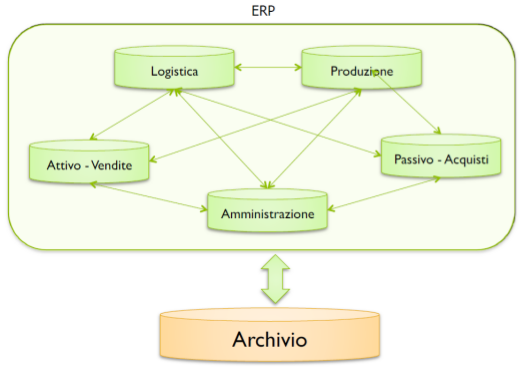
\includegraphics[scale=0.33]{ERP3}
	\end{figure}
\columnbreak
	\begin{figure}[H]
		\centering
		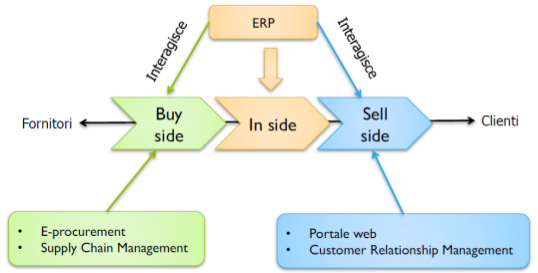
\includegraphics[scale=0.33]{ERP2}
	\end{figure}
	\begin{figure}[H]
		\centering
		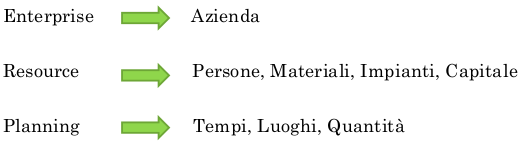
\includegraphics[scale=0.26]{ERP}
	\end{figure}
\end{multicols}

\noindent
\textit{\textbf{Amministrazione}}: modulo per le procedure di contabilità generale che supporta le attività amministrative (fatture, pagamenti e incassi) e produce informazioni di sintesi sull’andamento aziendale.

\noindent
\textit{\textbf{Logistica}}: procedure per la gestione dei materiali (materie prime, materiali di funzionamento, prodotti finiti). Si occupa della gestione interna della logistica e non del rapporto con clienti e fornitori.
\begin{itemize}
	\item Articoli: descrizione, caratteristiche operative, anagrafe fornitori, lotti riordino;
	\item Layout depositi aziendali: dislocazione dei depositi (interni o esterni all'azienda) e spostamento dei beni tra i depositi (flussi di carico/scarico).
\end{itemize}

\noindent
\textit{\textbf{Vendite Flusso Attivo}}:
	\begin{itemize}
		\item processi che permettono all’azienda di interagire con il cliente (gestione ordini);
		\item trattamento delle condizioni commerciali (listini, sconti e analisi dei costi aziendali);
		\item analisi per la valutazione della collocazione
		dell’azienda sul mercato;
		\item trattamento dei processi di gestione del rapporto col cliente:
		\begin{itemize}
			\item ricezione di ordini (valutazioni sul cliente prima di accettare, es.solvibilità);
			\item elaborazione degli ordini (valutazione priorità);
			\item evasione di ordini ed emissione di documenti di trasporto (interazione con il magazzino);
			\item fatturazione (interagisce con contabilità).
		\end{itemize}
	\end{itemize}
	\begin{figure}[H]
		\centering
		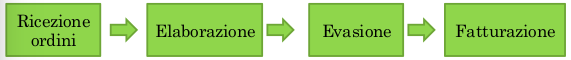
\includegraphics[scale=0.3]{Logistica}
	\end{figure}
	
\noindent
\textit{\textbf{Flusso Passivo}}: processi per l’interazione con i fornitori per approvvigionamento di materiali e lavorazioni/servizi esterni (molta correlazione con logistica e produzione).\\
Le principali funzioni di gestione riguardano condizioni commerciali (listini, sconti) e di rapporto con i fornitori.
\newline

\noindent
\textit{\textbf{Acquisti (gestione ordini)}}: raccolta delle richieste da parte della produzione e degli altri reparti (materiale di funzionamento), emissione di ordini al fornitore, ricezione documenti di consegna ed evasione di ordini fornitore, ricezione di fatture fornitore.
\begin{figure}[H]
	\centering
	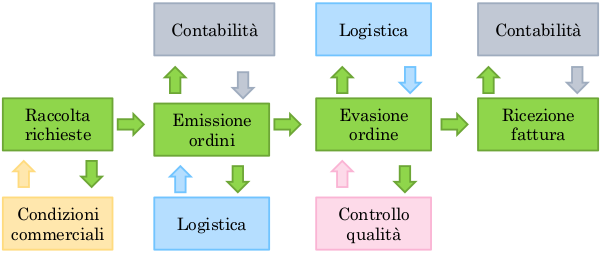
\includegraphics[scale=0.3]{Acquisti}
\end{figure}

\noindent
\textit{\textbf{Produzione}}: non esiste una soluzione unica per tutte le produzioni, ma diverse possibilità dipendenti. I produttori di \textit{ERP} forniscono sottosistemi di produzione verticalizzati. \textit{ERP} rispecchia il processo produttivo e viceversa (può aiutare ad ottimizzare il processo di produzione). Prima il processo produttivo influenzava il sistema informativo, adesso è il contrario.\\
Il modulo di produzione definisce dati tecnici: componenti per realizzare il prodotto (distinta base), risorse utilizzate (con cosa creo il prodotto) e processo produttivo (come creo il prodotto).\\
Il modulo di produzione svolge le seguenti funzioni:
\begin{itemize}
	\item pianificazione della produzione (per ottimizzare le risorse): richiesta di produzione (vincola cosa produrre), disponibilità di magazzino (tempi di approvvigionamento), disponibilità risorse (interne ed esterne);
	\item avanzamento e controllo della produzione: modellata come flusso di fasi (senza entrare nei dettagli), informazione su prelievo/versamento di materiali/prodotti, informazioni di avanzamento (inizio e fine di una fase).
\end{itemize}

\subsection*{SAP (multinazionale)}
\addcontentsline{toc}{subsection}{SAP (multinazionale)}
\textit{\textbf{SAP AG}} è una multinazionale europea per la
produzione di software. È una delle principali aziende al mondo nel settore degli \textit{ERP} e nelle soluzioni \textit{Enterprise}.
\newline

\noindent
Nel 1980 crea il linguaggio \textit{ABAP} (simile a COBOL/Fortran) per interrogare dati e interfacciarsi al linguaggio SQL (con tecnologia client-server) dei maggiori database relazionali. Nel 2000 integra soluzioni internet e Business Intelligence.
\\\\\\
I \textbf{moduli} dell'ERP di SAP sono:
\begin{itemize}
	\item \textit{\textbf{Sales and Distribution (SD) - Gestione Commerciale}}: colloca il prodotto/servizio sul mercato; comprende vendite spedizioni, trasporti, commercio estero, fatturazione.
	\item \textit{\textbf{Materials Management (MM) - Gestione Materiali}}: effettua la movimentazione dei materiali (pianificazione dei consumi, acquisti, controllo delle fatture, gestione degli stock, controllo di qualità, gestione del magazzino).
	\item \textit{\textbf{Product Planning (PP) - Pianificazione della Produzione}}: combina i fattori produttivi e li trasforma in beni e servizi (gestione della domanda, pianificazione delle capacità, della produzione e delle vendite).
	\item \textit{\textbf{Quality Management (QM) - Gestione della Qualità}}: pianificazione, controllo, ispezioni, avvisi, certificati (per verificare le variazioni della qualità).
	\item \textit{\textbf{Plant Maintenance (PM) - Manutenzione Impianti}}: pianificazione della manutenzione, la gestione degli oggetti tecnici e la gestione delle risorse.
	\item \textit{\textbf{Human Resources (HR) - Gestione delle Risorse Umane}}: reclutamento, allocazione, formazione, rilevazione delle presenze, gestione dei turni, calcolo delle retribuzioni.
	\item \textit{\textbf{Financial Accounting (FI) - Contabilità}}: rileva, elabora e comunica agli stakeholders i dati economici e quantitativi dell’azienda.
	\item \textit{\textbf{Controlling (CO) - Controllo di Gestione}}: accerta che le risorse siano acquisite ed impiegate in modo efficiente ed efficace (controllo degli
	ordini, controllo dei progetti, contabilità dei costi, analisi di profittabilità).
	\item \textit{\textbf{Asset Manager (AM) - Gestione Cespiti}}: gestisce i valori materiali e immateriali a utilità pluriennale.
	\item \textit{\textbf{Project System (PS) - Gestione Commesse}}: pianifica i progetti di ricerca e di sviluppo (pianificazione dei costi, pianificazione dei tempi, pianificazione delle capacità).
	\item \textit{\textbf{Workflow (WF)}}: gestisce i flussi di lavoro (gestione delle autorizzazioni, dei livelli di accesso e delle password).
	\item \textit{\textbf{Industry Solution (IS)}}: fornisce soluzioni settoriali per imprese specifiche (gestione degli immobili, la gestione dell’autoparco, la gestione del protocollo).
\end{itemize}


\section*{Il Portafoglio Operativo delle Società di Servizi}
\addcontentsline{toc}{section}{Il Portafoglio Operativo delle Società di Servizi}
Le società di servizi sono rappresentate da: settore bancario, settore assicurativo, servizi finanziari. Sono caratterizzate da un'alta intensità informativa (sia dei processi produttivi che dei prodotti/servizi).

\noindent
C'è sovrapposizione tra produzione e distribuzione:
\begin{itemize}
	\item \textit{processo produttivo}: predisposizione delle condizioni produttive (creare la capacità produttiva per erogare il servizio, anche con la stipulazione contratti con altri operatori, acquisto e apertura nuove filiali), attività di back-office (erogazione del servizio svolto in seguito ad un ordine ma non in presenza del cliente, come la valutazione del rischio di una polizza assicurativa);
	\item \textit{processo distributivo}: attività di front office (erogazione del servizio in presenza del cliente come l'attività di sportello della banca), ricerca della clientela (per la stipulazione dei contratti di servizio da parte dei clienti).
\end{itemize}

\textit{\textbf{Trattamento dell'informazione supportato dai sistemi informatici}}
\begin{itemize}
	\item \textit{Flusso degli ordini}: arrivo dell'ordine, produzione e distribuzione del servizio, post-vendita;
	\item \textit{Flusso di gestione della conoscenza (\textbf{knowledge management})}: elaborazione dell’informazione acquisita durante la produzione e l’erogazione del servizio; trasformazione in conoscenza accessibile alle attività operative e direzionali.
\end{itemize}
La gestione della conoscenza è vitale nelle società di servizi, dove essa rappresenta il vero capitale dell’azienda (\textit{vantaggio competitivo}). La gestione della conoscenza ha lo scopo di trasformare l’informazione non strutturata in informazione comprensibile a qualunque esperto. L’informazione non è strutturata, ad esempio:
\begin{itemize}
	\item la valutazione del rischio di una polizza assicurativa non è una formula (i fattori di rischio sono imprevedibili);
	\item la valutazione del premio è un’attività creativa basata su esperienza, intuito e sulle informazioni disponibili.
\end{itemize}
\textit{\textbf{Knowledge Worker}}: impiegato che svolge un lavoro intellettuale di natura decisionale. \MakeUppercase{è} una figura tipica delle società di servizi con elevato grado di personalizzazione o di trattativa con il cliente.

\subsection*{CRM e Aziende di Utility}
\addcontentsline{toc}{subsection}{CRM e Aziende di Utility}
I sistemi di \textit{Customer Relationship Management} supportano l’intero ciclo di rapporti con la clientela (marketing e pianificazione vendite, raccolta ordini e fatturazione, assistenza post-vendita). Questi sistemi informatizzano l'area \textit{sell-side} e attraverso Internet trasformano l'interazione tra aziende e clienti.

\noindent
Le aziende di \textbf{\textit{utility}} (forniscono gas, energia, acqua, telefono e simili) sono spinte ad uno sviluppo massiccio di sistemi a supporto dei contatti con il cliente per i seguenti motivi: clientela numerosa, rapporto continuativo nel tempo, sviluppo di canali virtuali (Web e call center), concorrenza crescente, necessità di sviluppare e mantenere un'offerta personalizzata. I conseguenti \textbf{vantaggi} sono: abbattimento dei costi di relazione, grande impatto sui profitti e buon grado di personalizzazione mantenendo i costi contenuti.

\noindent
Le funzioni principali dei sistemi \textit{CRM} sono i sistemi di gestione degli ordini (es. Amazon), sistemi di automazione delle forze di vendita (venditori dotati di pc per gestione di offerte e ordini), sistemi di assistenza telefonica (call center).

\subsection*{CRM e Business Intelligence}
\addcontentsline{toc}{subsection}{CRM e Business Intelligence}
Gli strumenti di \textit{Business Intelligence} sono applicazioni che estraggono informazioni dai sistemi di supporto alla produzione per elaborarle e fornire supporto all’apparato decisionale (nel portafoglio decisionale servono ad analizzare lo stato dell'azienda e prendere decisioni). Si occupano di passare da dati a informazione sintetica.\\
L’architettura dei sistemi di \textit{Business Intelligence} comprende: una serie di \textit{data warehouse} e una serie di \textit{data mart}.



\chapter*{Ingegneria Sociale}
\addcontentsline{toc}{chapter}{Ingegneria Sociale}
\textit{\textbf{Ingegneria Sociale}}: Una manipolazione della naturale tendenza alla fiducia dell’essere umano, architettata e realizzata dall’ingegnere sociale con l’obiettivo \textit{ottenere informazioni} che permettano di raggiungere l'obiettivo prefissato.
\begin{itemize}
	\item \textit{\textbf{Sociale}}: perché coinvolge e studia il comportamento umano.
	\item \textit{\textbf{Ingegneria}}: è necessario pianificare la situazione per raggiungere i propri obiettivi (come nell’hacking, la maggior parte del lavoro è nella preparazione, piuttosto che nel tentativo stesso). L’ingegnere sociale programma l’attacco anticipando le domande che il bersaglio può porgli in modo da \textit{avere sempre la risposta pronta}.
\end{itemize}
\textit{\textbf{Ingegnere Sociale}}: sceglie la vittima, sviluppa una causa plausibile per ottenere subito confidenza, stabilisce un obiettivo minimo, costruisce il rapporto su simpatia o altre tecniche per influenzare la vittima, sviluppa risposte per superare le possibili obiezioni, prevede una via d'uscita per non bruciare l'origine del contatto.

\noindent
\textit{\textbf{FootPrinting}}: l’ingegnere sociale prima di compiere il gesto criminoso comincia a raccogliere informazioni sul sistema da colpire (può durare mesi). In questo tempo studia e impara: i sistemi di comunicazione aziendale, funzionamento della posta interna, organigramma aziendale, giorni e orari di pulizia, frequenta gli uffici (es. consegna buste, caffè, ecc.), conosce e dialoga col personale (addetti alla sicurezza, segretarie, sistemisti, ecc.), cerca di ottenere informazioni (manda e-mail, telefonate), finge di essere un utente inesperto che ha smarrito al password, manda un'offerta di un nuovo firewall per aumentare il sistema di sicurezza.

\noindent
\textit{\textbf{Phreaker}}: furono i primi utilizzatori dell'ingegneria sociale per ottenere informazioni vitali dalle compagnie telefoniche. Utilizzavano la rete telefonica
sfruttando i sistemi e i dipendenti dell’azienda erogatrice del servizio.

\noindent
\textit{\textbf{Sicurezza}}: non è un prodotto acquistabile ma un processo evolutivo che coinvolge l’organizzazione nella sua interezza; però spesso è solo un'\textit{illusione} poiché, se si rubano soldi o beni qualcuno si accorge che
sono spariti. Ma quando si rubano informazioni nessuno lo nota, perché restano comunque in possesso della vittima.

\noindent
\textit{\textbf{Informazioni}}: sono memorizzate nei computer sono gestite da operatori umani che molto spesso ignorano le procedure di sicurezza. La sicurezza non è un problema di tecnologia, bensì di persone e gestione.

\noindent
Le \textit{\textbf{Vittime Preferite}} sono le persone che: non hanno niente da perdere nel fornire una informazione sensibile, sottostimano il valore delle informazioni, pensano che seguire le basilari regole per la sicurezza delle informazioni sia una perdita di tempo, non valutano le conseguenze delle loro azioni.
\newline

\noindent
L'\textit{ingegneria sociale} spesso funziona perché è più facile dell'hacking, non richiede dispositivi particolari, ha un costo basso e un basso rischio, lascia poche tracce, è efficace, non diventa obsoleta ed è poco conosciuta dalle vittime.\\
Questi attacchi possono avere successo perché di solito le persone non conoscono bene le pratiche di sicurezza.

\section*{Fasi dell'Attacco}
\addcontentsline{toc}{section}{Fasi dell'Attacco}
\begin{itemize}
	\item \textit{\textbf{Fase Fisica}}: raccolta di informazioni attraverso persone (\textit{shoulder surfing}), documenti (supporti digitali distrutti, stampe di dati sensibili), luoghi (\textit{dumpster diving}).
	\item \textit{\textbf{Fase Psicologica}}: impersonificazione, carpire le informazioni utili attraverso la persuasione.
\end{itemize}

\subsection*{Fase Fisica}
\addcontentsline{toc}{subsection}{Fase Fisica}
\textit{\textbf{Strumenti Essenziali}}: buona memoria per raccogliere le informazioni, telefoni, fax, scanner, stampanti, server di posta, cooperazione, argomenti e ragioni per giustificare l'azione (più la persona target è vicina alle informazioni e più forti devono essere le argomentazioni).

\noindent
\textit{\textbf{Obiettivi dell'Attacco}}: password, obiettivi fisici (modem, server), help desk(processo per fornire supportoriguardo prodotti/servizi informatici ed elettronici).

\noindent
I \textit{\textbf{Metodi di Attacco}} sono due (serve la giusta combinazione di entrambi):
\begin{itemize}
	\item interazione con altre persone o azioni svolte senza l'ausilio di mezzi tecnologici;
	\item attacchi svolti con l'ausilio della tecnologia.
\end{itemize}
\textit{\textbf{Attacchi mediante interazione umana}}: richiesta diretta di informazioni, truffe telefoniche, rovistare nella carta straccia (\textit{dumpster diving}) che viene ancora stampata in grandi quantità, rovistare negli hard disk dismessi, richiesta di informazioni per un falso sondaggio, sbirciare alle spalle (\textit{shoulder surfing}).

\noindent
\textit{\textbf{Attacchi Tecnologici}}: attacchi diretti alsistema (creazione di un nuovo account e aggiungere privilegi o diritti di accesso a un account esistente), esecuzione di un programma malintenzionato (trojan), attivazione di un piano di \textit{phishing} (loghi contraffatti), intercettazioni telefoniche, invio di mail contenenti malware o false proposte (\textit{Nigeriam Scam}, mail in cui si parla di somme di denaro da trasferire chiedendo informazioni sensibili), microfoni, webcam, tastiere (\textit{KeyGhost}, un dispositivo che cattura qualsiasi cosa venga digitata sulla tastiera).\\
Altre tecniche utilizzate sono le finestre di pop-up (chiedere nuovamente username e password per qualche problema di rete), spam e catene di S.Antonio (non causano danni ma riducono la produttività), siti web (offrire qualcosa di gratis o la possibilità di vincere qualcosa), file scambiati tramite peer-to-peer (una volta scaricati, il sistema viene utilizzato come stazione di comunicazione e attacco per aggressioni verso l'esterno per comunicare dati sensibili).
\newline

\noindent
\textit{\textbf{Metodi Classici}}: fingersi un collega, fingersi un fornitore o un tutore dell'ordine, fingersi un nuovo assunto che chiede aiuto, fingersi un fabbricante di sistemi che offre aggiornamenti o patch al sistema, usare una falsa finestra pop-up per ottenere credenziali, inviare programmi o patch gratis da installare, inviare malware, far registrare ad un sito web fasullo, modificare intestazione dei fax (per far sembrare che provengano dall'interno), fingere di essere di un'altra sede dell'azienda per avere accessi a posta elettronica o altri dati.

\noindent
\textit{\textbf{Reverse Social Engineering}}: offrire aiuto in caso di problemi, poi fare in modo che il problema si presenti realmente, convincendo così la vittima a chiedere aiuto.
\newline

\noindent
\textit{\textbf{Trucchi Fondamentali}}:
\begin{itemize}
	\item \textit{domanda "mina antiuomo"}: si pone la domanda "mina", se il bersaglio risponde senza cambiare tono di voce significa che non è scettico e si può porre la vera domanda senza insospettirlo.
	\item per non insospettire, non bisogna mai interrompere la conversazione una volta ottenuta l'informazione chiave (proseguire come se nulla fosse).
\end{itemize}
\textit{\textbf{Ingegnerizzare se stessi}}: diventare qualcun altro (meglio al telefono), vestirsi in base all'occasione, imparare a parlare in base al proprio ruolo, dire ciò che il bersaglio vuole sentirsi dire (imparare il più possibile su di esso), saper mentire.

\subsection*{Fase Psicologica}
\addcontentsline{toc}{subsection}{Fase Psicologica}
\textit{\textbf{Sicurezza e Fiducia}}: il primo obiettivo dell'ingegnere sociale è creare fiducia nella vittima, a quel punto può scattare la trappola, che può sfruttare le conoscenze informatiche dell'aggressore (la sicurezza si basa sulla fiducia).

\noindent
\textit{\textbf{Peopleware}}: l'anello debole non è la persona ma la naturale tendenza a credere alla parola altrui. L'ingegnere sociale fa levo sui comportamenti (naturali, sollecitati, forzati) che tutti mostriamo.

\noindent
\textit{\textbf{Obiettivi della fase psicologica}}: osservare il comportamento delle persone, imparare come pensano, localizzare le debolezze umane, imparare quali parole usare quando si parla a certe persone.

\noindent
\textit{\textbf{Su cosa agire}}: l'ingegnere sociale fa leva sui bisogni primari dell’uomo per far sì che la propria richiesta venga accettata. I \textit{\textbf{bisogni primari}} sono: fisiologici (funzionali al mantenimento psicofisico dell’uomo), sicurezza (essere fuori pericolo, stabilità, protezione), appartenenza (essere accettati da altri), stima (ottenere approvazione/riconoscimento).\\
I \textit{\textbf{bisogni secondari}} sono: cognitivi (conoscere, comprendere, esplorare), estetici (simmetria, ordine, bellezza), autorealizzazione (trasformare in realtà il potenziale inespresso), trascendenza (aiutare altri a realizzare il loro potenziale).

\noindent
\textit{\textbf{Tendenze base della natura umana}}: autorevolezza (tendenza a cedere quando una persona autorevole fa una richiesta), simpatia (tendenza ad obbedire quando chi fa la richiesta suscita simpatia),ricambiare (tendenza ad obbedire automaticamente ad una richiesta quando viene dato o promesso qualcosa di valore), coerenza (tendenza a dire di sì dopo aver sposato pubblicamente una causa per evitare di apparire inaffidabili), convalida sociale (tendenza ad obbedire quando, in questo modo, si fa quello che fanno gli altri), scarsità (tendenza a dire di sì quando si crede che l’oggetto cercato stia scarseggiando e altri siano in competizione per averlo).

\noindent
\textit{\textbf{Caratteristiche delle Vittime}}: paura delle conseguenze, senso di colpa, sentimentalismo, ritenere che l’azione possa dare loro un vantaggio, tendenza a dare fiducia agli altri, dovere morale identificazione con l'ingegnere sociale, attitudine all'aiuto, convinzione della propria non vulnerabilità (i nuovi assunti sono una preda facile).

\noindent
\textit{\textbf{Persuasione}}: la finalità non è quella di forzare un individuo a fare qualcosa ma quella di aumentare la sua volontaria condiscendenza alle richieste altrui. La vittima viene guidata sul percorso scelto dall’attaccante, lasciandole credere di avere il controllo totale della situazione.

\noindent
\textit{\textbf{Strumenti di Persuasione}}: impersonificazione, conformità (conformarsi al giudizio degli altri), diffusione di responsabilità (ritengono che l’azione riduca le loro responsabilità), accattivarsi la fiducia altrui e usare la cortesia.


\chapter*{Ingegneria dei Processi Gestionali}
\addcontentsline{toc}{chapter}{Ingegneria dei Processi Gestionali}
I \textit{\textbf{processi}} (\textit{business process}) rappresentano il modo di operare di un’azienda. Le \textit{\textbf{tecnologie informatiche}} e di rete trasformano il modo di operare di un’azienda e quindi i processi. Si ha la necessità di integrare l’innovazione informatica con l’innovazione organizzativa per migliorare costi, tempi o qualità (l'innovazione tecnologica ha ricadute sull’organizzazione aziendale).\\
I processi possono essere:
\begin{itemize}
	\item \textit{materiali} (flusso di materiali e attività);
	\item \textit{informativi} (flusso di informazioni input/output);
	\item \textit{Business Process} o \textit{Processo Aziendale} (un insieme strutturato di attività, finalizzato alla realizzazione di un risultato di interesse per l’organizzazione).
\end{itemize}

\noindent
\textit{\textbf{Business Process Reengineering (BPR)}}: necessità di correlare un’innovazione radicale di processi e organizzazione aziendale con un massiccio uso di informatica.

\noindent
\textit{\textbf{Business Process (BP)}}: un processo aziendale è formato da attività, realizzate come processi materiali o processi informativi, che sono collegate fra loro nel tempo e nello spazio e sono svolte dalle risorse di un’azienda. Partendo da input definiti, le attività producono
un output utilizzato dai clienti.\\
Sono flussi di attività interfunzionali che concatenano: competenze commerciali (marketing), competenze tecniche (produzione), competenze generali (approvvigionamento).\\
Un \textit{Business Process} è definito come una tupla \textbf{BP = (A, I, O, C)}, dove:
\begin{itemize}
	\item \textbf{A} = attività (operazioni fisiche o di decisioni manageriali con esecuzione coordinata);
	\item \textbf{I} = input (materie prime e risorse aziendali oppure informazioni se è un processo decisionale);
	\item \textbf{O} = output (oggetti fisici, beni immateriali, servizi);
	\item \textbf{C} = clienti (destinatari dell’output del processo).
\end{itemize}
\textit{\textbf{Catena del Valore di Porter}}: l'azienda è vista come una successione di attività (un processo) finalizzate a produrre valore per il cliente che viene misurato dal prezzo che il cliente è disposto a pagare.
\begin{figure}[H]
	\centering
	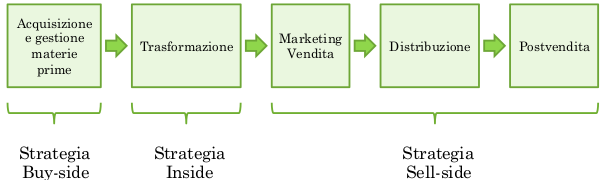
\includegraphics[scale=0.45]{Cat}
\end{figure}
\noindent
\textit{\textbf{Trasformazione dei Processi - Strategia Buy-Side}}: trasforma il processo nelle varie fasi di ricerca del fornitore, definizione di prezzi e condizioni, ordinazione, ricezione dei beni e servizi ordinati. L'obiettivo è ridurre il costo di transazione e del materiale stesso. La trasformazione si appoggia a sistemi di \textit{E-procurement} e infrastrutture internet.

\noindent
\textit{\textbf{Trasformazione dei Processi - Strategia In-Side}}: trasformazione dei processi interni all’impresa per ridurre i costi di funzionamento e della durata dei processi e migliorare la qualità e il servizio al cliente. La trasformazione si appoggia a sistemi \textit{ERP} e infrastrutture internet.

\noindent
\textit{\textbf{Trasformazione dei Processi - Strategia Sell-Side}}: orientata ai processi di marketing, vendita, distribuzione e servizio post-vendita/assistenza al cliente. Si ha un maggiore valore del prodotto percepito dal cliente e un abbattimento dei costi di transazione. La trasformazione si appoggia a sistemi \textit{CRM} e infrastrutture internet.
\newline

\noindent
\textit{\textbf{Classificazione dei processi}}
\begin{itemize}
	\item \textit{Processi intersettoriali}: sono generici e descrivono le pratiche di vari settori (gestione/acquisto materie \dots).
	\item \textit{Processi settoriali}: distinguono i vari settori (nel settore sanitario ci sono processi di ricovero, di cura \dots);
	\item \textit{Processi aziendali}: processi di una specifica azienda o di una sua parte (specializzazione dei processi settoriali);
	\item \textit{Processi normativi e best practice}: processi di riferimento; Best practice derivano dal confronto tra processi diversi e descrivono come dovrebbero essere nelle migliori aziende del settore.
\end{itemize}
\textit{\textbf{Scomposizione dei processi} (dettaglia i processi per livelli di approfondimento successivi)}
\begin{itemize}
	\item \textit{Macroprocessi}: primo livello di segmentazione di un’azienda (es. la \textit{Catena del Valore di Porter});
	\item \textit{Processi}: illustrano il modo di operare dell’azienda;
	\item \textit{Fasi (Sottoprocessi)}: illustrano il modo in cui un processo è implementato (una fase è una tappa del processo);
	\item \textit{Attività}: livello minimo di analisi normalmente adottato nello studio dei processi; le attività sono determinate scomponendo i processi secondo una logica sequenziale;
	\item \textit{Operazioni}: passi elementari per eseguire una certa attività (quasi mai usate).
\end{itemize}


\section*{Griglia Metodologica}
\addcontentsline{toc}{section}{Griglia Metodologica}
La \textit{griglia metodologica} è orientata a una strategia integrata di progettazione dei processi. Essa comprende:
\begin{itemize}
	\item descrizione della variabili di analisi (\textit{variabili organizzative});
	\item descrizione delle \textit{fasi di analisi};
	\item identificazione degli strumenti a supporto delle attività di analisi (es. diagrammi di flusso).
\end{itemize}

\subsection*{Variabili Organizzative}
\addcontentsline{toc}{subsection}{Variabili Organizzative}
La trasformazione dei processi deve integrare innovazione tecnologica e organizzativa. L'azione è necessaria su tutte le variabili organizzative che, insieme alla tecnologia informatica, sono le leve attraversi i quali sono trasformati i progetti.

\noindent
Le variabili di progettazione integrata dei processi sono:
\begin{itemize}
	\item \textit{Flusso delle attività}: sequenza delle attività attraverso cui è svolto il processo;
	\item \textit{Organizzazione del processo}: divisione operativa del lavoro nell’ambito del processo, cioè come i processi sono mappati sui ruoli (può indicare parallelizzazione o accorpamento delle attività);
	\item \textit{Competenza delle risorse umane che operano nel processo}: fondamentale per la trasformazione del processo a seguito di un'innovazione tecnica;
	\item \textit{Sistema di misurazione e controllo delle prestazioni usato per governare il processo e valutare gli attori aziendali che lo eseguono}.
\end{itemize}

\subsubsection*{Variabile 1 - Flussi delle Attività}
Il flusso delle attività determina: la durata del processo (dipende dal numero di attività), il livello di servizio (dipende dal grado di flessibilità), la qualità del prodotto (insieme a tecnologia e risorse umane).

\noindent
La modellazione dei flussi può essere condotta a diversi livelli: \textit{schemi di sequenza} (indicano solo la sequenza delle attività che formano un processo) e \textit{schemi più ricchi} (indicano gli attori coinvolti, gli eventi che determinano le attività e le informazioni utilizzate).

\noindent
Gli elementi della modellazione dei flussi sono:
\begin{itemize}
	\item natura del flusso: fisico, informativo, controllo;
	\item attività: tipo, durata, volumi, tecnologie;
	\item sequenza attività: alternative nella sequenza (eventuale struttura di controllo);
	\item attori: tipologia, azioni svolte sul flusso;
	\item eventi:tipologia, temporizzazione, conseguenza dell'evento sull'attività (avvia, ferma, modifica);
	\item oggetti: natura (fisico, informativo), profilo temporale (informazioni permanenti/temporanee);
\end{itemize}

\subsubsection*{Variabile 2 - Organizzazione}
L’organizzazione è una determinante strutturale della prestazione del processo e si dividono in due tipi:
\begin{itemize}
	\item organizzazioni parcellizzate (per compiti ripetitivi e semplici con alti volumi);
	\item organizzazioni piatte con mansioni articolate (per lavori complessi e volumi limitati).
\end{itemize}
Per descrivere l'organizzazione si possono usare: organigrammi, tabelle di proprietà, Linear Responsibility Charting (\textit{LRC}).
\newline

\noindent
\textit{\textbf{Organigramma}}: Gerarchia delle responsabilità e delle autorità di un'organizzazione con vari livelli di dettaglio.

\noindent
\textit{\textbf{Tabella delle Proprietà} (logiche/quantitative)}: indica le proprietà \textit{logiche} (descrizione del mandato, elenco dei compiti assegnati e dei processi svolti) e \textit{quantitative} (organici e volumi del lavoro) delle strutture.

\begin{multicols}{2}
\textit{\textbf{Linear Responsibility Charting (LRC)}}: offre una visione tabellare della responsabilità organizzativa che integra quella dell’organigramma. Per ciascun processo, specifica il ruolo svolto da ogni struttura nel processo.

\noindent
Il ruolo può essere: \textbf{D} (decide, autorizza), \textbf{E} (esegue le attività), \textbf{A} (dà assistenza operativa e supporto), \textbf{I} (sistematicamente informato).
\columnbreak
\begin{figure}[H]
	\centering
	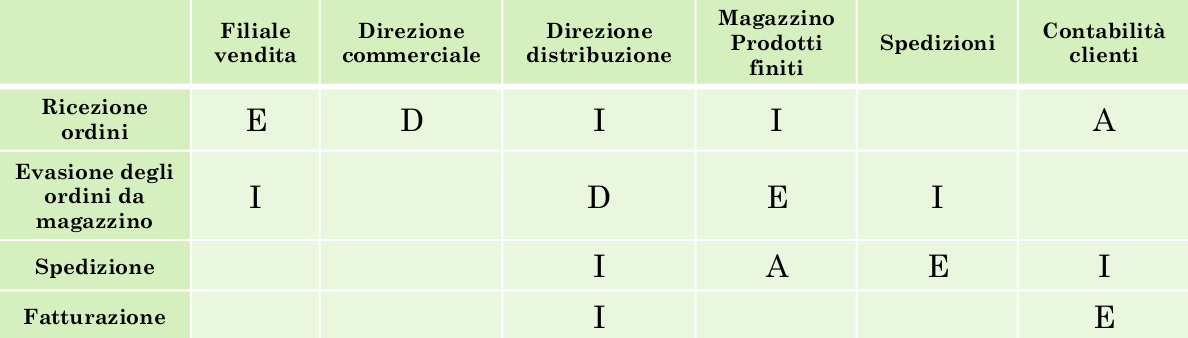
\includegraphics[scale=0.20]{LRC}
\end{figure}
\end{multicols}

\subsubsection*{Variabile 3 - Risorse Umane}
Le risorse umane determinano la differenza tra il risultato effettivo di un processo e il massimo risultato teoricamente possibile. L’innovazione tecnologica causa la necessità di avere a disposizione figure professionali specializzate:
\begin{itemize}
	\item creandole internamente riconvertendo il personale si possono avere problemi gestionali (superamento dell'avversione al cambiamento e accettazione delle nuove tecnologie);
	\item acquisite sul mercato (reperimento complesso e costoso).
\end{itemize}

\subsubsection*{Variabile 4 - Sistema di Misurazione delle Prestazioni}
Ogni processo è governato da un sistema di misurazione delle prestazioni che comprende:
\begin{itemize}
	\item \textit{sistema di pianificazione e controllo}: fissa gli obiettivi di efficienza e efficacia del processo e li controlla periodicamente;
	\item \textit{sistema di promozione e incentivazione}: fissa gli obiettivi del processo come vendite e soddisfazione del cliente;
	\item \textit{sistema dei valori}: posiziona gli obiettivi dell'azienda e decide i valori rispetto a cui incentivare (in un processo orientato all’utente, è prioritaria la soddisfazione del cliente).
\end{itemize}

\subsection*{Fasi di Analisi}
\addcontentsline{toc}{subsection}{Fasi di Analisi}
Rappresentano i passi logici attraverso cui si svolge l’analisi dei processi.
\begin{itemize}
	\item Fasi (approccio \textit{bottom-up} al miglioramento del processo esistente): rilevazione della situazione esistente, confronto con altre imprese e diagnosi dei problemi, ridisegno dei processi.
	\item Fasi (approccio \textit{top-down}): disegno del processo con applicazione di criteri di ottimizzazione noti, analisi della situazione esistente per capire cos'è necessario per attuare il progetto.
\end{itemize}
In ogni fase vengono analizzate le variabili organizzative appena descritte.

\subsubsection*{Fase 1 - Rilevazione della Situazione Esistente}
\begin{itemize}
	\item \textbf{Passo 1} - \textit{Identificazione dei
	macroprocessi}: identificazione dei processi usando un opportuno modello (catena del valore, checklist, best practice) e rilevazione delle proprietà fondamentali:
	\begin{itemize}
		\item quali sono i clienti del processo (esterni / interni);
		\item tipo di processo (inside/buy-side/sell-side);
		\item input del processo (materie prime, competenze);
		\item output del processo (prodotto/servizio fornito al cliente).
	\end{itemize}
	\item \textbf{Passo 2} - \textit{Dettaglio dei processi}: composizione dei processi in fasi e attività,
	documentata da:
	\begin{itemize}
		\item diagrammi gerarchici (processo $\rightarrow$ fasi $\rightarrow$ attività);
		\item diagrammi di flusso (flussi fisici e/o informativi);
		\item schede che descrivono le proprietà di processi, fasi, attività, operazioni.
	\end{itemize}
	\item \textbf{Passo 3} - \textit{Incrocio processi/unità
		organizzative}: analisi della relazione fra strutture organizzative e processi da tre punti di vista:
	\begin{itemize}
		\item rilevazione delle strutture organizzative (organigrammi);
		\item definizione dei ruoli delle strutture nei processi (\textit{LRC});
		\item mappatura delle attività delle strutture nel flusso dei processi (opportuni diagrammi di flusso chiamati \textit{Responsibility Activity Diagram – RAD}).
	\end{itemize}
	\item \textbf{Passo 4} - \textit{Valutazione del processo}: definizione dei parametri di funzionamento e giudizio sul valore dei prodotti. Comprende:
	\begin{itemize}
		\item giudizio sul processo da parte degli esecutori (costo del processo in termini di tempo usato dalle risorse e tempo di completamento del processo);
		\item giudizio sul processo da parte dei clienti interni o esterni in termini di:
		\begin{itemize}
			\item utilità/valore (prezzo che il cliente è disposto a pagare);
			\item livello del servizio (puntualità e velocità);
			\item qualità (contenuto del prodotto e assenza di difetti).
		\end{itemize}
	\end{itemize}
\end{itemize}

\subsubsection*{Fase 2 - Confronto e Diagnosi}
\begin{itemize}
	\item \textbf{Passo 1} - \textit{Confronto quantitativo e parametrazione}: per il confronto tra prestazioni di aziende concorrenti secondo alcuni parametri (produttività, livello di servizio, durata attività);
	\item \textbf{Passo 2} - \textit{Confronto qualitativo}: misurare le cause della diversità rispetto a valori di mercato (fase decisiva per la scelta di eventuali cambiamenti organizzativi). Si tratta di esaminare le variabili organizzative per individuare le aree in cui una diversità può indicare un legame causa-effetto (evidenziazione delle differenze di modello organizzativo e tecnologico).
\end{itemize}

\subsubsection*{Fase 3 - Ridefinizione}
\begin{multicols}{2}
\begin{itemize}
	\item Definizione della \textit{vision} che dà una rappresentazione sintetica degli elementi fondamentali della soluzione: illustra la nuova struttura del flusso di attività e gli aspetti più significativi della configurazione delle variabili gestionali.
	\item Analisi del cambiamento: specificazione dell’impatto organizzativo del progetto (incrocia le variabili organizzative con gli stackholder) e valutazione di rischi, benefici, tempi e costi del cambiamento.
\end{itemize}
\columnbreak
\begin{figure}[H]
	\centering
	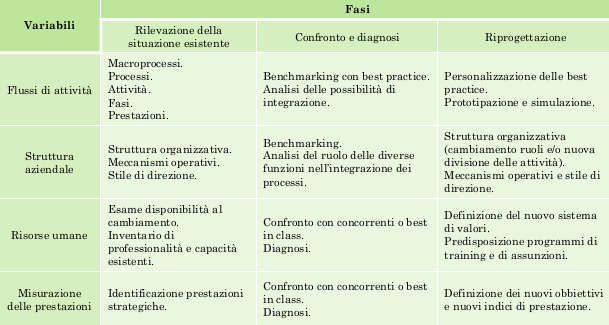
\includegraphics[scale=0.3]{Griglia}
\end{figure}
\end{multicols}

\section*{Trasformazione dei Processi}
\addcontentsline{toc}{section}{Trasformazione dei Processi}
L’applicazione delle tecnologie dell’informazione ha come effetto l’integrazione inter-funzionale o inter-organizzativa dei processi che offre la possibilità di condividere informazioni prima non disponibili e di eseguire congiuntamente attività prima svolte separatamente dalle singole unità (le organizzazioni possono ottenere benefici consistenti).\\
L’\textit{informatica} consente una maggiore integrazione inter-funzionale e inter-organizzativa per due ragioni fondamentali: aumenta la disponibilità di informazioni e supporta l’esecuzione dei compiti individuali di natura decisionale.



\chapter*{Business Process Model and Notation (BPMN)}
\addcontentsline{toc}{chapter}{Business Process Model and Notation (BPMN)}


\section*{Modellazione di processi e dati}
\addcontentsline{toc}{section}{Modellazione di processi e dati}



\chapter*{Data Warehousing}
\addcontentsline{toc}{chapter}{Data Warehousing}
L'\textit{informatica in azienda} era vista come una scienza di supporto che rende più rapide ed economiche le operazioni di gestione delle informazion (ma non crea ricchezza). Adesso invece i sistemi informatici si sono trasformati da semplici strumenti per migliorare l'efficienza dei processi a elementi centrali dell'organizzazione aziendale (rivoluziona i processi).\\
l'\textit{informatica ha un duplice ruolo}: 
\begin{itemize}
	\item tecnologia di supporto alla gestione del Sistema Informativo;
	\item disciplina organizzativa che influenza processi, servizi e struttura aziendale.
\end{itemize}
I motivi principali per migliorare il Sistema Informativo sono tre:
\begin{itemize}
	\item \textbf{Trasformazione dell'Economia}: l’economia moderna è basata sulle conoscenze e sull'informazione ed è caratterizzata da una breve vita dei prodotti che richiede decisioni tempestive;
	\item \textbf{Trasformazione dell'Impresa}: per operare con profitto in un sistema economico altamente competitivo le aziende hanno bisogno di una struttura flessibile in grado di reagire rapidamente alle mutate situazioni esterne/interne;
	\item \textbf{Globalizzazione}: con l’allargamento dei mercati a livello mondiale nasce l’esigenza del controllo di mercati a larga scala.
\end{itemize}
Per il portafoglio direzionale si parla anche di \textbf{\textit{Business Intelligence}}: disciplina che consente a chi deve decidere in azienda di capire, attraverso soluzioni software, i fattori chiave del business e conseguentemente di prendere le migliori decisioni in quel momento. Si parla di piattaforma perchè neccessita di un'apposita infrastruttura hardware e software di supporto.\\
Il ruolo chiave di una piattaforma di \textit{business intelligence} è la trasformazione dei dati aziendali in informazioni fruibili a diversi livelli di dettaglio.\\
L'\textit{informazione} è un bene a valore crescente e costituisce la materia prima trasformata dai sistemi informativi. Spesso la disponibilità di troppi dati rende difficile (se non impossibile) estrapolare le informazioni veramente importanti (\textbf{dati $\neq$ informazione}).\\
Per ogni azienda è fondamentale poter disporre in maniera rapida e completa delle informazioni necessarie al processo decisionale; l'aumento esponenziale del volume dei dati operazionali ha reso il calcolatore l’unico supporto adatto e il ruolo dell’informatica è passato da passivo strumento per la registrazione delle operazioni a fattore decisivo per l'individuazione di elementi critici dell’organizzazione e potenziali aree di business.\\\\
Negli anni '80 nascono i sistemi di supporto alle decisioni (\textbf{DSS, Decision Support System}): l'insieme delle tecniche e degli strumenti informatici atti a estrapolare informazioni da un insieme di dati memorizzati su supporti elettronici.


\section*{Introduzione al Data Warehousing}
\addcontentsline{toc}{section}{Introduzione al Data Warehousing}
Uno scenario tipico è quello di una grande azienda, con tante filiali, i cui dirigenti vogliono monitorare il contributo dato da ciascuna di esse al rendimento dell'impresa. Un \textit{raccoglitore di informazioni} (\textit{\textbf{DataWarehouse}}) che integra e riorganizza i dati provenienti da sorgenti distinte e li rende disponibili per analisi e valutazioni finalizzate alla pianificazione e al processo decisionale.

Mescolare interrogazioni \textit{analitiche} e \textit{transazionali} di routine porta a inevitabili rallentamenti che rendono insoddisfatti entrambi gli utenti. \MakeUppercase{è} necessario separare l'elaborazione di tipo analitico (\textbf{OLAP}, \textit{On-Line Analytical Processing}) da quella legata alle transazioni (\textbf{OLTP}, \textit{On-Line Transactional Processing}), costruendo un raccoglitore di informazione che integri i dati provenienti da sorgenti di varia natura.
Alcune aree di utilità sono: commercio, manifattura, servizi finanziari, trasporti, telecomunicazioni, sanità $\dots$
\\\\
\textit{\textbf{Data Warehousing}}: collezione di metodi, tecnologie e strumenti di ausilio al \textit{knowledge worker} (dirigente, amministratore, gestore, analista) per condurre analisi dei dati finalizzate all'attuazione di processi decisionali e al miglioramento del patrimonio informativo.
\\
Il processo di \textit{warehousing} possiede le seguenti caratteristiche:
\begin{itemize}
	\item \textit{accessibilità} a utenti con conoscenze limitate di informatica e strutture dati;
	\item \textit{integrazione dei dati} sulla base di un modello standard dell'impresa;
	\item \textit{flessibilità di interrogazione} per trarre il massimo vantaggio dal patrimonio informativo esistente;
	\item \textit{sintesi} per permettere analisi mirate ed efficaci;
	\item \textit{rappresentazione multidimensionale} per offrire all’utente una visione intuitiva e manipolabile delle informazioni;
	\item \textit{correttezza e completezza} dei dati integrati.
\end{itemize}
Un \textit{\textbf{Data Warehouse}} è una collezione di dati di supporto per il processo decisionale che presenta le seguenti caratteristiche: orientata ai soggetti di interesse, integrata e consistente, rappresentativa dell'evoluzione temporale (c'è un ricco contenuto storico a differenza dei DB operazionali, la "fotografia" dei dati ad un certo istante di tempo non può essere aggiornata), non volatile.
\newline

\noindent
Le interrogazioni sono di due tipi:
\begin{itemize}
	\item \textbf{OLTP}: le interrogazioni eseguono transazioni che leggono e scrivono un ridotto numero di record da diverse tabelle;
	\item \textbf{OLAP}: le interrogazioni effettuano un’analisi dinamica e multidimensionale che richiede la scansione di un’enorme quantità di record per calcolare un insieme di dati numerici di sintesi che quantifichino le prestazioni dell’azienda.
\end{itemize}
Le \textbf{architetture} devono avere i seguenti requisiti:
\begin{itemize}
	\item \textit{separazione}: l’elaborazione analitica e quella transazionale devono essere mantenute il più possibile separate;
	\item \textit{scalabilità}: l’architettura hardware e software deve essere facilmente ridimensionabile a fronte della crescita nel tempo dei volumi di dati da gestire degli utenti da soddisfare;
	\item \textit{estendibilità}: poter accogliere nuove applicazioni e tecnologie senza riprogettare integralmente il sistema;
	\item \textit{sicurezza}: il controllo sugli accessi è essenziale a causa della natura strategica dei dati memorizzati;
	\item \textit{amministrabilità}: la complessità dell’attività di amministrazione non deve risultare eccessiva.
\end{itemize}

\subsection*{Architettura a 2 Livelli}
\addcontentsline{toc}{subsection}{Architettura a 2 Livelli}
\begin{multicols}{2}
	\begin{figure}[H]
		\centering
		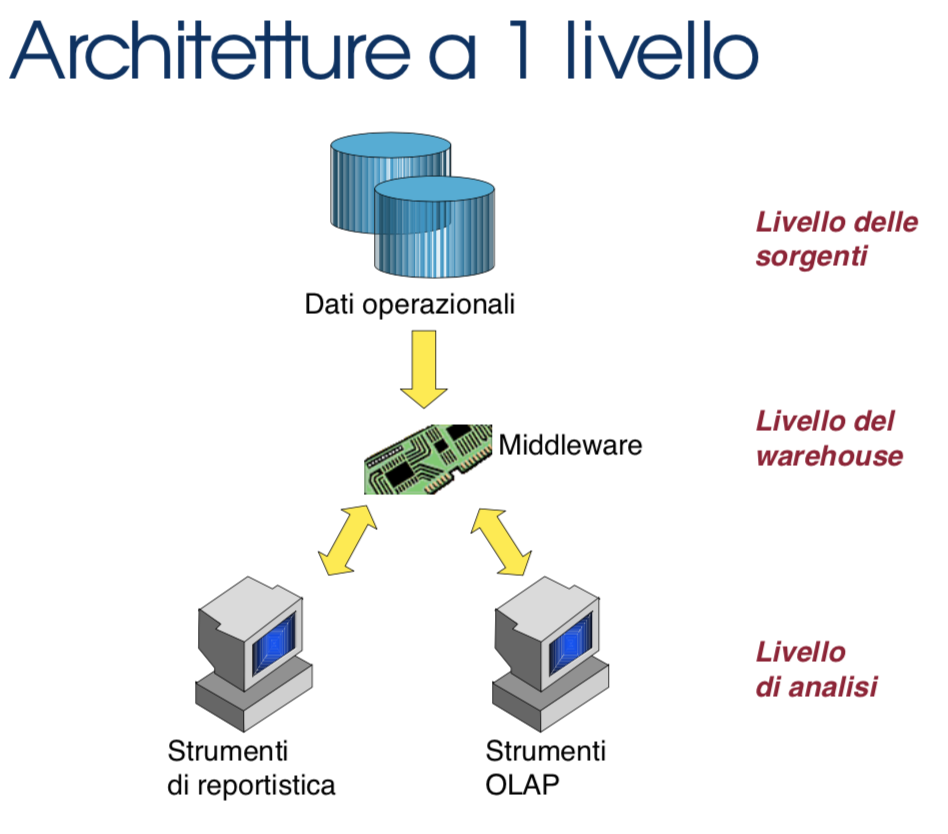
\includegraphics[scale=0.32]{Arch1Liv}
	\end{figure}
\columnbreak
	\begin{figure}[H]
		\centering
		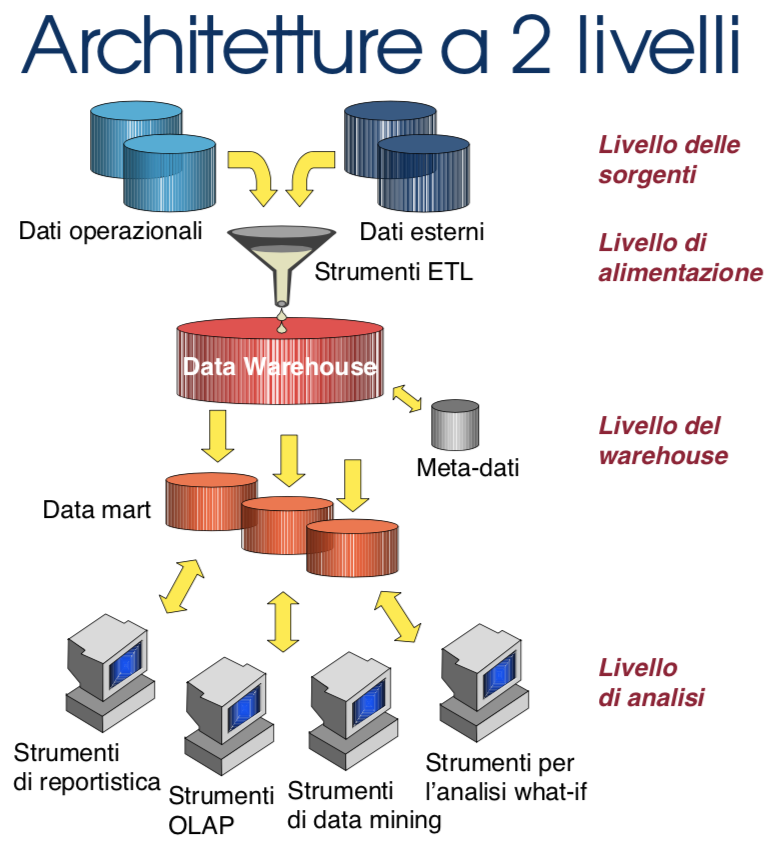
\includegraphics[scale=0.32]{Arch2Liv}
	\end{figure}
\end{multicols}
\textit{\textbf{Data Mart}}: un sottoinsieme o un’aggregazione dei dati presenti nel DW primario, contenente l’insieme delle informazioni rilevanti per una particolare area del business, divisione dell’azienda o categoria di soggetti. Ci sono due tipi di \textit{data mart}:
\begin{itemize}
	\item \textit{dipendenti}: sono quelli alimentati dal DW primario; utili in aziende medio-grandi poichè delineano i contorni delle informazioni necessario ad un certo tipo di utenti e permettono di raggiungere migliori prestazioni (dimensioni inferiori);
	\item \textit{indipendenti}: alimentati direttamente dalle sorgenti; l'assenza di un DW primario snellisce le fasi progettuali ma determina uno schema complesso di accesso ai dati (rischio di inconsistenze tra i data mart).
\end{itemize}
L'\textit{architettura a 2 livelli} presenta i seguenti \textbf{vantaggi}:
\begin{itemize}
	\item  informazione di buona qualità sempre disponibile anche quando, per motivi tecnici, non è disponibile l'accesso alle sorgenti;
	\item l'interrogazione analitica non inferisce con la gestione delle transazioni
	\item l'organizzazione logica del DW si basa sul modello relazionale (le sorgenti offrono modelli relazionali o semi-strutturali);
	\item c'è una distanza temporale tra sistemi OLTP (trattano dati correnti e al massimo livello di dettagli) e sistemi OLAP (operano su dati storici e di sintesi);
	\item è possibile impiegare tecniche per ottimizzare le prestazioni per applicazioni di analisi e reportistica.
\end{itemize}

\subsection*{Architettura a 3 Livelli}
\addcontentsline{toc}{subsection}{Architettura a 3 Livelli}
\begin{multicols}{2}
	L'\textit{architettura a 3 livelli} ha il livello dei dati riconciliati, il cui vantaggio principale è che crea un modello di dati comune e di riferimento per l'intera azienda. Introduce una separazione netta tra le problematiche legate all'estrazione e integrazione dei dati e quelle inerenti l'alimentazione del DW.
	I dati riconciliati, però, introducono un'ulteriore ridondanza rispetto ai dati sorgente.
	\newline
	
	\textit{\textbf{Dati Riconciliati}}: dati operazionali ottenuti dopo il processo di integrazione e ripulitura dei dati sorgente, quindi dati integrati, consistenti, corretti, volatili, correnti e dettagliati.
	\newline
	
	Il ruolo degli strumenti di \textit{Extraction}, \textit{Transformation} and \textit{Loading} è quello di alimentare una sorgente dati singola, dettagliata, esauriente e di alta qualità che possa a sua volta alimentare il DW (\textit{riconciliazione}).\\
	La riconciliazione avviene due volte durante il processo di alimentazione del DW: quando viene popolato per la prima volta, e periodicamente quando viene aggiornato (estrazione, pulitura, trasformazione e caricamento).
	\columnbreak
	\begin{figure}[H]
		\centering
		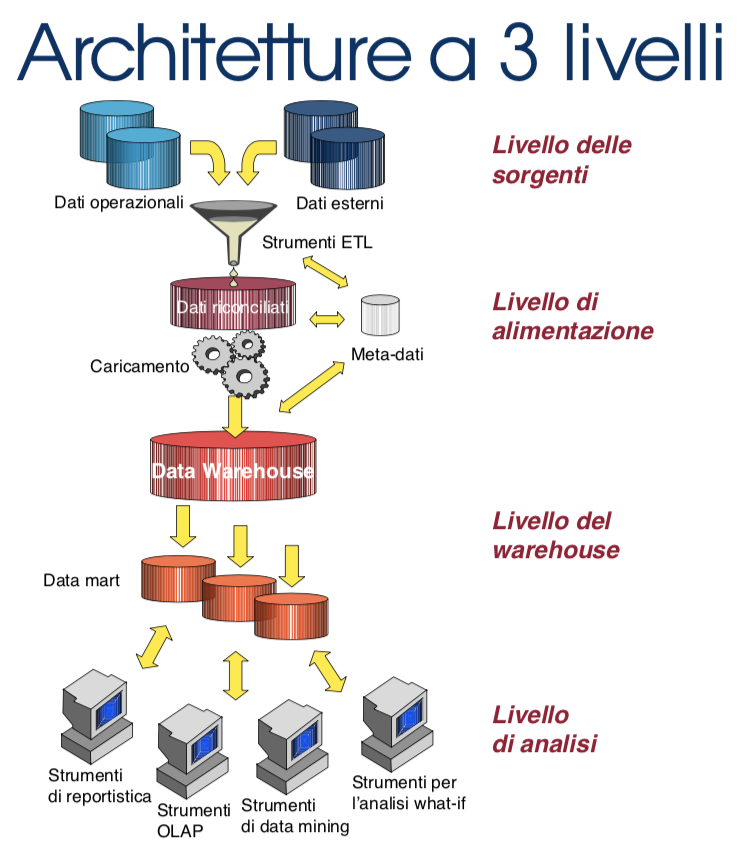
\includegraphics[scale=0.42]{Arch3Liv}
	\end{figure}
\end{multicols}
\noindent
\textit{\textbf{Estrazione}}: i dati rilevanti vengono estratti dalle sorgenti e vengono scelti principalmente in base alla loro qualità. L'\textit{estrazione statica} aviene quando il DW deve essere popolato per la prima volta (fotografia dei dati operazionali). L'\textit{estrazione incrementale} viene usata per l’aggiornamento periodico del DW (cattura i cambiamenti avvenuti nelle sorgenti dall’ultima estrazione).

\noindent
\textit{\textbf{Pulitura}}: si incarica di migliorare la qualità dei dati delle sorgenti (dati duplicati, incosistenza tra valori, dati mancanti, valori impossibili o errati, valori inconsistenti per le diverse convenzioni o errori di battitura).
\newline

\noindent
\textit{\textbf{Trasformazione}}: converte i dati dal formato operazionale sorgente a quello del DW. La corrispondenza è complicata dalla presenza di fonti eterogenee, che richiede una complessa fase di integrazione (es. formati differenti per lo stesso dato).
\newline

\noindent
\textit{\textbf{Caricamento}}: i dati vengono caricati nel DW con \textit{Refresh} (i dati vengono riscritti integralmente, sostituendo quelli precedenti, come nel caso della prima popolazione del DW) e con \textit{Update} (i soli cambiamenti occorsi nei dati sorgente vengono aggiunti nel DW).

\section*{Il modello Multidimensionale}
\addcontentsline{toc}{section}{Il modello Multidimensionale}
\MakeUppercase{è} il fondamento per la rappresentazione e l'interrogazione dei dati nei DW. I \textbf{\textit{fatti di interesse}} sono rappresentati in \textit{cubi} in cui:
\begin{itemize}
	\item ogni \textit{cella} contiene \textit{misure} numeriche che quantificano il fatto da diversi punti di vista;
	\item ogni \textit{asse} rappresenta una \textit{dimensione} di interesse per l’analisi;
	\item ogni \textit{dimensione} può essere la radice di una \textit{gerarchia} di attributi usati per aggregare i dati memorizzati nei cubi base.
\end{itemize}
\begin{multicols}{2}
	\begin{figure}[H]
		\centering
		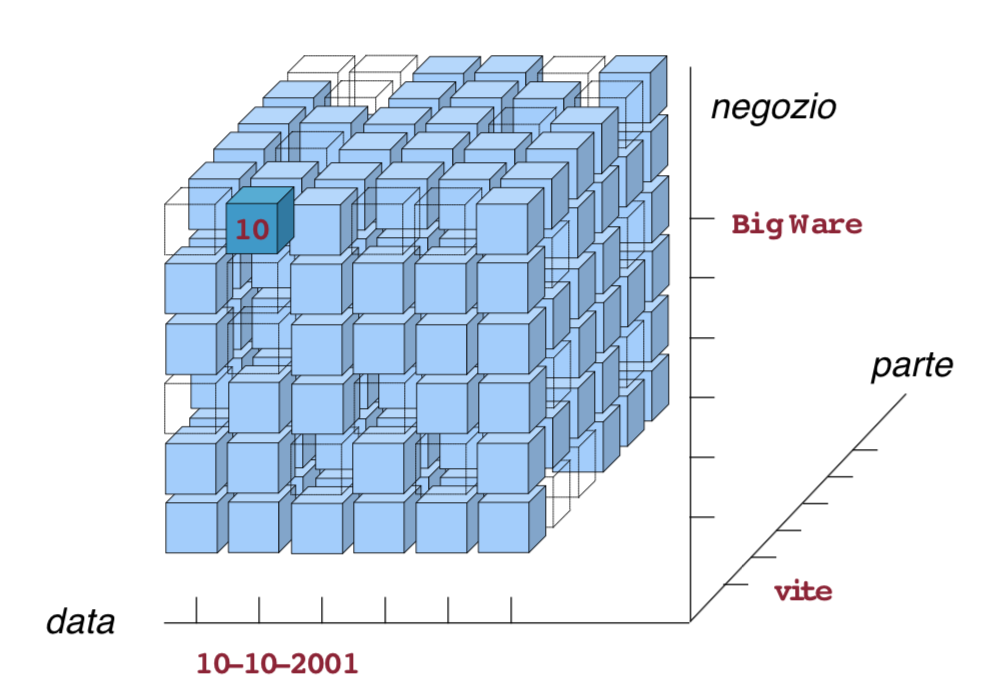
\includegraphics[scale=0.35]{CuboVendite}
	\end{figure}
	\columnbreak
	\begin{figure}[H]
		\centering
		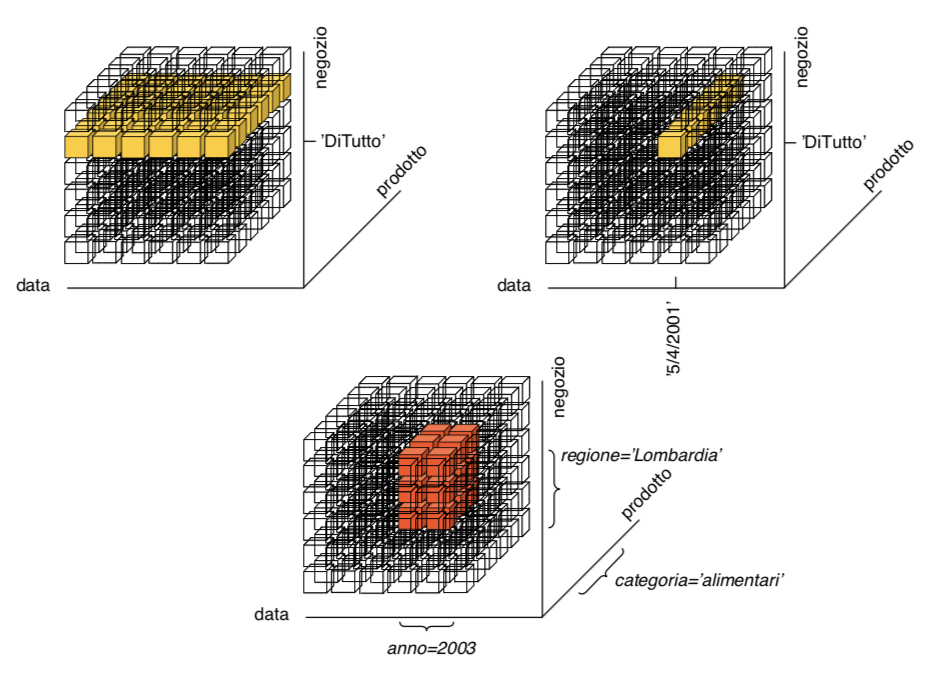
\includegraphics[scale=0.38]{Slicing}
	\end{figure}
\end{multicols}
Una volta che i dati sono stati ripuliti, integrati e trasformati, occorre capire come trarne il massimo vantaggio informativo. Esistono in sostanza tre approcci per l'interrogazione di un DW da parte degli utenti finali:
\\\\
\textit{\textbf{Reportistica}}: non richiede conoscenze informatiche; orientato agli utenti che hanno necessità di accedere, a intervalli di tempo predefiniti, a informazioni strutturate in modo pressoché invariabile.
\begin{multicols}{2}
	\begin{figure}[H]
		\centering
		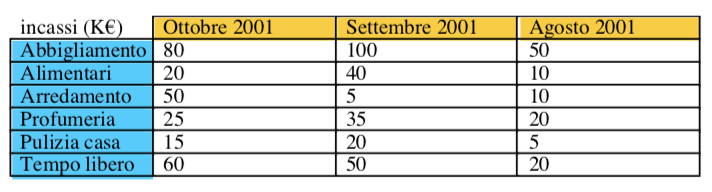
\includegraphics[scale=0.5]{Reportistica}
	\end{figure}
\columnbreak
	\begin{figure}[H]
		\centering
		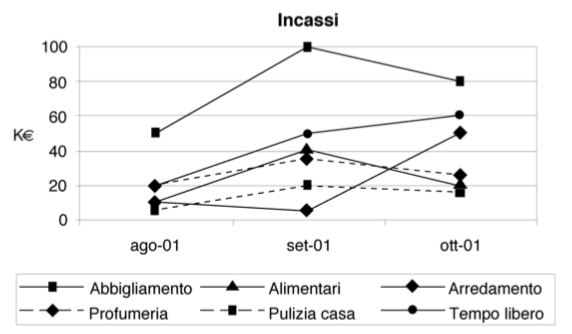
\includegraphics[scale=0.4]{Reportistica2}
	\end{figure}
\end{multicols}

\noindent
\textit{\textbf{OLAP}}: l'utente deve ragionare in modo multidimensionale e deve conoscere l’interfaccia dello strumento grafico utilizzato (orientamento verso utenti non esperti di informatica); \MakeUppercase{è} il metodo principale per ottenere le informazioni contenute in un DW. Consente di analizzare ed esplorare interattivamente i dati sulla base del modello multidimensionale. Gli utenti OLAP sono in grado di costruire attivamente una sessione di analisi complessa in cui ciascun passo effettuato è conseguenza dei risultati ottenuti al passo precedente.\\
Una sessione OLAP consiste in un \textit{percorso di navigazione} che rappresenta l'analisi di uno o più fatti di interesse sotto diversi aspetti e a diversi livelli di dettaglio. \MakeUppercase{è} sequenza di interrogazioni spesso formulate non direttamente, ma per differenza rispetto all’interrogazione precedente. Ogni passo della sessione di analisi è scandito dall’applicazione di un \textit{operatore OLAP} che trasforma l’ultima interrogazione formulata in una nuova interrogazione. Il risultato è di tipo multidimensionale (rappresenta i dati in modo tabellare).
\\\\
\textit{\textbf{Data Mining}}: richiede all’utente la conoscenza dei principi che stanno alla base degli strumenti utilizzati. \MakeUppercase{è} un'attività orientata a scoprire informazioni nascoste nei dati. Il data mining raccoglie tecniche di intelligenza artificiale e pattern recognition per aiutare l’utente nella ricerca di pattern: è sufficiente indicare cosa e dove si vuole ricercare (ricerche di mercato, studio dell'efficacia del marketing, segmentazione di mercato, analisi delle abitudini di acquisto, pianificazione aziendale, modellazione degli investimenti, rilevamento di attività fraudolente, valutazione delle categorie di rischio).
\begin{itemize}
	\item \textit{Regole Associative}: consentono di individuare i gruppi di affinità tra oggetti attraverso lo studio delle abitudini di acquisto per la pubblicità mirata e l’organizzazione della merce sugli scaffali (\textit{market-basket analysis}).
	\item \textit{Clustering}: significa raggruppare gli oggetti in un ridotto numero di insiemi (\textit{cluster}) che caratterizzino al meglio la popolazione (es. segmentazione della
	clientela in categorie).
	\item \textit{Alberi Decisionali}: usati per la comprensione di un particolare fenomeno poiché permettono di classificare, in ordine di importanza, le cause che portano al verificarsi di un evento (es. valutazione delle categorie di rischio dei clienti per le società che concedono mutui e prestiti).\\
	\item \textit{Serie Temporali}: individuazione di pattern ricorrenti o atipici in sequenze di dati complesse (identificazione di schemi associati alla crescita dei titoli di borsa, rilevazione anomalie nel sistema di monitoraggio, analisi percorsi di navigazione in siti web).
	\newline
\end{itemize}

\noindent
\textit{\textbf{ROLAP} (Relational OLAP)}: giustificato dall’enorme lavoro svolto sul modello relazionale, dalla diffusa esperienza aziendale sull’utilizzo di basi di dati relazionali e dall’elevato livello di prestazioni e flessibilità dei DBMS relazionali.\\
Si presenta la necessità di elaborare tipologie specifiche di schemi che permettano di traslare il modello multidimensionale sul modello relazionale. C'è il problema delle prestazioni (costose operazioni di join tra tabelle di elevate dimensioni).
\\\\
\textit{\textbf{MOLAP} (Multidimensional OLAP)}: è basato su un modello logico ad hoc sul quale i dati e le operazioni multidimensionali possono essere direttamente rappresentati. I dati vengono fisicamente memorizzati in vettori e l’accesso è di tipo posizionale.\\
Il \textit{\textbf{vantaggio}} dell’approccio \textit{MOLAP} rispetto a quello \textit{ROLAP} è che le operazioni multidimensionali sono realizzabili in modo semplice e naturale, senza necessità di ricorrere a join (prestazioni ottime). Non esistendo ancora uno standard per il modello logico multidimensionale, le diverse implementazioni \textit{MOLAP} hanno poco in comune (solo l'utilizzo di tecnologie ottimizzate per trattare il problema della sparsità).
\\\\
La \textit{\textbf{qualità di un processo}} misura la sua aderenza agli obiettivi degli utenti ed è caratterizzata da: \textit{accuratezza} (conformità tra valore memorizzato e quello reale), \textit{attualità} (dato memorizzato non obsoleto), \textit{completezza} (non mancano informazioni), \textit{consistenza} (rappresentazione uniforme dei dati), \textit{disponibilità} (dati facilmente disponibili all'utente), \textit{tracciabilità} (possibilità di risalire alla fonte di ciascun dato), \textit{chiarezza} (dati facilmente interpretabili).


\section*{Il Ciclo di Vita del Data Warehouse}
\addcontentsline{toc}{section}{Il Ciclo di Vita del Data Warehouse}
Molte organizzazioni mancano di esperienza e capacità per affrontare le sfide implicite nei progetti di data warehousing. Una delle cause principali è la mancata adozione di una \textit{approccio metodologico}, che minimizza i rischi di insuccesso essendo basato su un’analisi costruttiva degli errori commessi. Il rischio di ottenere un risultato insoddisfacente è particolarmente alto a causa delle elevatissime aspettative degli utenti. Una larga parte della responsabilità della riuscita del progetto ricade sulla qualità dei dati sorgente e sulla lungimiranza, disponibilità e dinamismo del personale dell’azienda.

\subsection*{Approccio Top-Down}
Analizza i bisogni globali dell’intera azienda e pianifica lo sviluppo del DW per poi progettarlo e realizzarlo nella sua interezza.
\begin{multicols}{2}
	\noindent
	Il \textit{vantaggio} di questo approccio è il seguente:
	\begin{itemize}
		\item promette ottimi risultati poiché si basa su una visione globale dell’obiettivo e garantisce di produrre un DW consistente e ben integrato.
		\item 
		\item 
		\item 
		\item 
		\item 
	\end{itemize}
	\columnbreak
	Gli \textit{svantaggi} di questo approccio sono i seguenti:
	\begin{itemize}
		\item il preventivo con costi onerosi e lunghi tempi di realizzazione scoraggiano la direzione dall’intraprendere il progetto;
		\item affrontare contemporaneamente l’analisi e la riconciliazione di tutte le sorgenti di interesse è complesso;
		\item prevedere a priori le esigenze delle diverse aree aziendali è pressoché impossibile, e il processo di analisi rischia di subire una paralisi;
		\item il fatto di non prevedere la consegna a breve termine di un prototipo non permette agli utenti di verificare l’utilità del progetto e ne fa scemare l’interesse e la fiducia.
	\end{itemize}
\end{multicols}

\subsection*{Approccio Bottom-Up}
Il DW viene costruito in modo incrementale, assemblando iterativamente più data mart, ciascuno dei quali incentrato su un insieme di fatti collegati a uno specifico settore aziendale e di interesse per una certa categoria di utenti.
\begin{multicols}{2}
	\noindent
	I \textit{vantaggi} di questo approccio sono i seguenti:
	\begin{itemize}
		\item determina risultati concreti in tempi brevi;
		\item non richiede elevati investimenti finanziari;
		\item permette di studiare solo le problematiche relative al data mart in oggetto;
		\item fornisce alla dirigenza un riscontro immediato sull’effettiva utilità del sistema in via di realizzazione;
		\item mantiene costantemente elevata l’attenzione sul progetto
	\end{itemize}
	\columnbreak
	Lo \textit{svantaggio} di questo approccio è il seguente:
	\begin{itemize}
		\item determina una visione parziale del dominio di interesse.
		\item 
		\item 
		\item 
		\item 
		\item 
	\end{itemize}
\end{multicols}
\noindent
Il primo \textit{data mart} da prototipare deve essere quello che gioca il ruolo più strategico per l’azienda, deve ricoprire un ruolo centrale per l’intero DW, si deve appoggiare su fonti dati già disponibili e consistenti. Il ciclo di sviluppo è il seguente:
\begin{multicols}{2}
	\noindent
	\textit{\textbf{Definizione obiettivi e pianificazione}}: individuazione degli obiettivi, stima delle dimensioni del sistema, scelta dell'approccio per la costruzione, valutazione dei costi e del valore aggiunto, analisi dei rischi e delle aspettative.
	\\
	\textit{\textbf{Progettazione dell'infrastruttura}}: si analizzano e si comparano le possibili soluzioni architetturali valutando le tecnologie e gli strumenti disponibili.
	\\
	\textit{\textbf{Progettazione e sviluppo dei data mart}}: ogni iterazione comporta la creazione di un nuovo data mart e nuove applicazioni, che vengono integrate nel sistema di data warehousing.
	\columnbreak
	\begin{figure}[H]
		\centering
		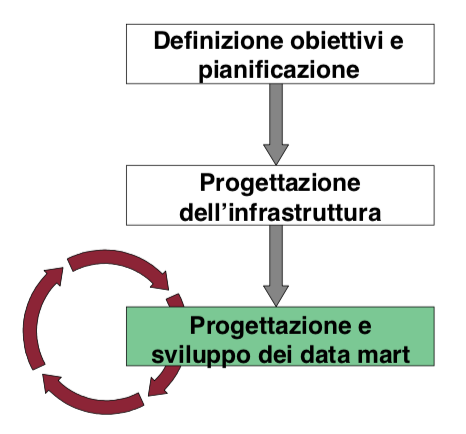
\includegraphics[scale=0.45]{CicloSviluppo}
	\end{figure}
\end{multicols}

\subsection*{Analisi e Riconciliazione delle Sorgenti Operazionali}
\addcontentsline{toc}{subsection}{Analisi e Riconciliazione delle Sorgenti Operazionali}
Il progettista, confrontandosi con gli esperti del dominio applicativo, acquisisce una buona conoscenza delle sorgenti operazionali:
\begin{itemize}
	\item \textit{\textbf{Ricognizione}}: esame approfondito degli schemi locali per comprendere appieno il dominio applicativo;
	\item \textit{\textbf{Normalizzazione}}: per correggere gli schemi locali al fine di modellare in modo più accurato il dominio applicativo.
\end{itemize}
\textit{Ricognizione} e \textit{normalizzazione} devono essere svolte anche qualora sia presente una sola sorgente dati; se esistono più sorgenti, l’operazione dovrà essere ripetuta per ogni singolo schema.
\newline

\noindent
L’\textit{\textbf{integrazione}} di un insieme di sorgenti dati eterogenee (basi di dati relazionali, file dati, sorgenti legacy) consiste nell’individuazione delle corrispondenze tra i concetti rappresentati e nella risoluzione dei conflitti evidenziati, per creare un unico schema globale i cui elementi possano essere correlati con i corrispondenti elementi degli schemi locali (\textit{mapping}).\\
Deve anche identificare l’insieme di concetti distinti e memorizzati in schemi differenti che sono correlati attraverso proprietà semantiche (\textit{interschema}). Per ragionare sui concetti negli schemi delle diverse sorgenti è necessario utilizzare un unico formalismo.
Ci possono essere diverse relazioni tra concetti comuni:
\begin{itemize}
	\item \textit{\textbf{identità}}: utilizzati stessi costrutti, concetto modellato dallo stesso punto di vista e non vengono commessi errori di specifica;
	\item \textit{\textbf{equivalenza}}: sono stati utilizzati costrutti diversi (ma equivalenti) e non ci sono errori di specifica o diversità di percezione;
	\item \textit{\textbf{comparabilità}}: i costrutti utilizzati e i punti di vista dei progettisti non sono in contrasto tra loro;
	\item \textit{\textbf{incompatibilità}}: gli schemi sono in contrasto a causa dell’incoerenza nelle specifiche;
\end{itemize}
Ci sono quattro \textit{\textbf{fasi dell'integrazione}}:
\begin{itemize}
	\item \textit{preintegrazione}: viene definita la strategia di integrazione;
	\item \textit{Comparazione degli schemi}: analisi comparativa dei diversi schemi per identificare le correlazioni e i conflitti tra i concetti.
	\item \textit{Allineamento degli schemi}: risoluzione dei conflitti evidenziatisi al passo precedente, che si ottiene applicando primitive di trasformazione agli schemi sorgenti o allo schema riconciliato temporaneamente definito (cambio di nomi e tipi degli attributi, modifica delle dipendenze). Non sempre i conflitti possono essere risolti, poiché derivano da inconsistenze di base del sistema informativo; in questo caso la soluzione deve essere discussa con gli utenti che dovranno fornire indicazioni su qual è la più fedele interpretazione del mondo reale.
	\item \textit{Fusione e ristrutturazione degli schemi}: gli schemi allineati vengono fusi a formare un unico schema riconciliato (sovrapposizione dei concetti comuni a cui saranno collegati i rimanenti concetti degli schemi locali). Poi si applicano altre trasformazioni per migliorare la struttura dello schema riconciliato rispetto a completezza, minimalità e leggibilità.
\end{itemize}

\subsection*{Analisi dei Requisiti}
\addcontentsline{toc}{subsection}{Analisi dei Requisiti}
La fase di analisi dei requisiti ha l’obiettivo di raccogliere le esigenze di utilizzo del data mart espresse dagli utenti finali. Ha un’importanza strategica poiché influenza le decisioni da prendere riguardo: schema concettuale dei dati, specifiche delle applicazioni per l’analisi dei dati, architettura del sistema, linee guida per la manutenzione e l’evoluzione del sistema.\\
La “fonte” principale da cui attingere i requisiti sono i futuri utenti del data mart (\textit{business users}). La differenza nel linguaggio usato da progettisti e utenti rende il dialogo difficile e a volte infruttuoso. Per gli aspetti più tecnici, saranno gli amministratori del sistema informativo a fungere da riferimento per il progettista (in questo caso, i requisiti che dovranno essere catturati riguardano principalmente vari vincoli sul sistema di data warehousing).\\\\
Esistono due tipi di \textit{\textbf{Interviste}}:
\begin{itemize}
	\item a \textit{\textbf{piramide} (approccio induttivo)}: si parte da domande dettagliate per poi ampliare l’argomento con domande aperte che richiedono risposte più generali (per superare lo scetticismo dell'intervistato, poiché non richiede un forte coinvolgimento).
	\item a \textit{\textbf{imbuto} (approccio deduttivo)}: si parte da domande molto generali per poi restringere l’argomento a temi specifici. Utile nel caso in cui l’intervistato sia emozionato (le domande generali non prevedono risposta sbagliata e alleviano la tensione).
\end{itemize}
\begin{multicols}{2}
	\begin{figure}[H]
		\centering
		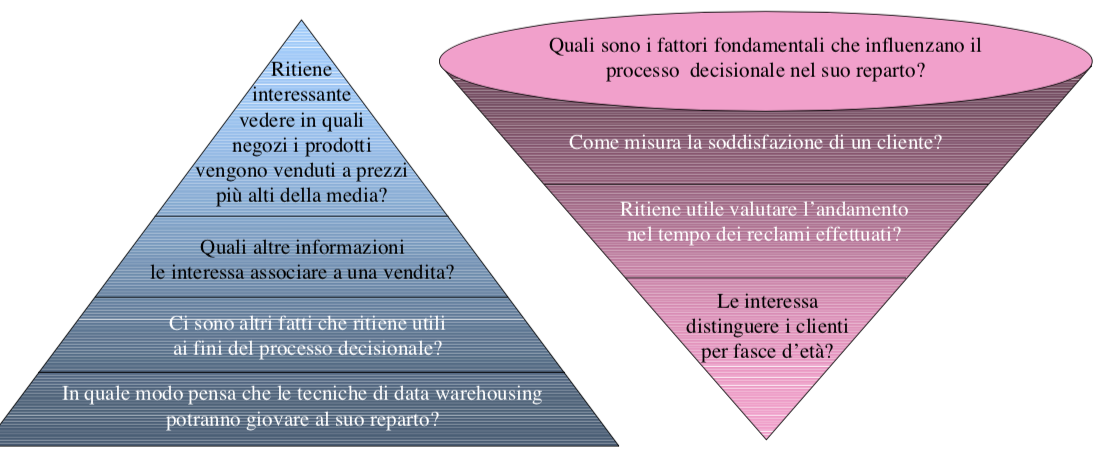
\includegraphics[scale=0.42]{Piramide}
	\end{figure}
\columnbreak
	\begin{figure}[H]
		\centering
		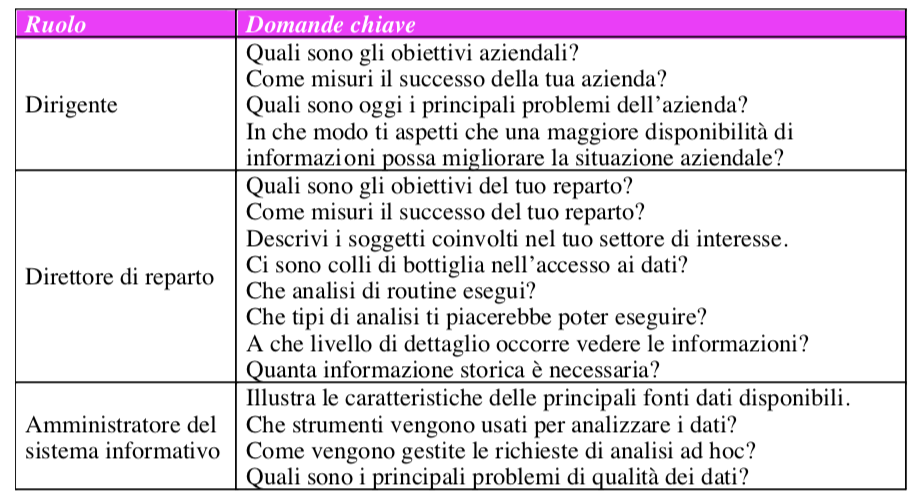
\includegraphics[scale=0.42]{Domande}
	\end{figure}
\end{multicols}
\noindent
I \textit{\textbf{fatti}} sono i concetti su cui gli utenti finali del data mart baseranno il processo decisionale; ogni \textit{fatto} descrive una categoria di eventi che si verificano in azienda. Fissare le dimensioni di un fatto è importante poiché significa determinarne la \textit{granularità} (il più fine livello di dettaglio a cui i dati saranno rappresentati). La scelta della granularità di un fatto nasce da un compromesso tra due esigenze contrapposte: raggiungere un'elevata flessibilità d'utilizzo e conseguire buone prestazioni. Per ogni fatto occorre definire l’\textit{intervallo di storicizzazione} (l’arco temporale che gli eventi memorizzati dovranno coprire).\\
Il riconoscimento di fatti (dimensioni e misure) è strettamente collegato all’identificazione di un \textit{carico di lavoro preliminare} che può essere espresso in linguaggio naturale (utile per valutare la granularità dei fatti e iniziare ad affrontare il problema dell’aggregazione).
\begin{multicols}{2}
	\begin{figure}[H]
		\centering
		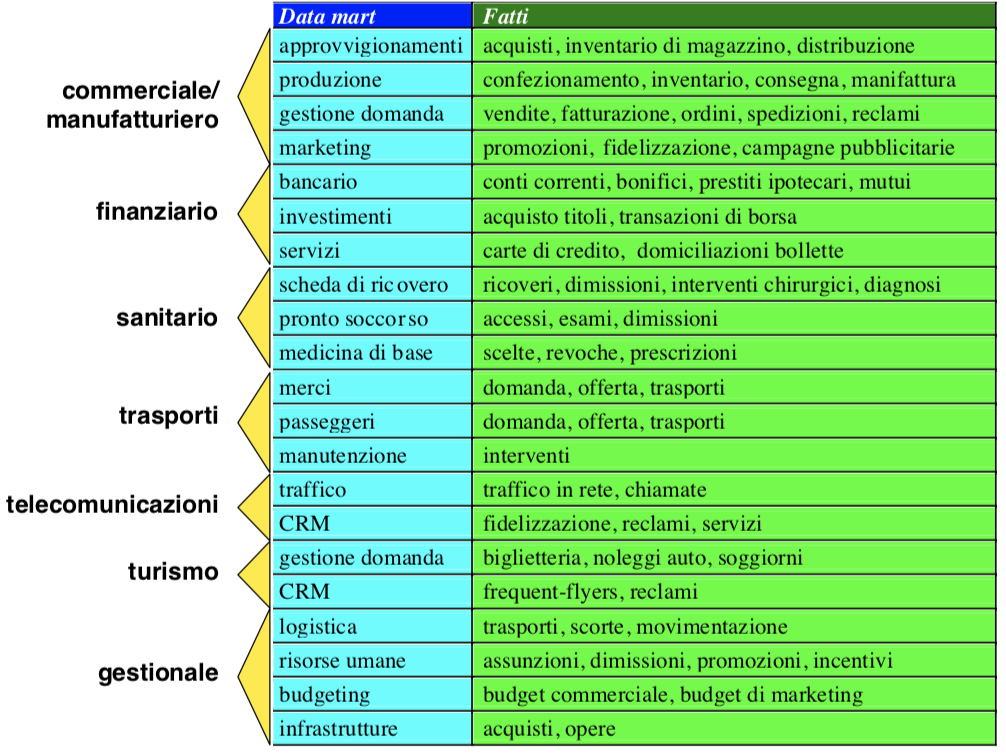
\includegraphics[scale=0.45]{Fatti}
	\end{figure}
	\columnbreak
	\begin{figure}[H]
		\centering
		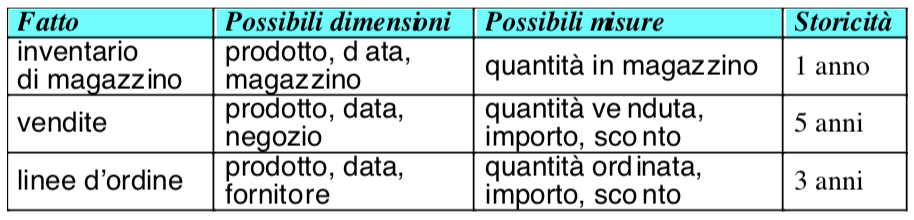
\includegraphics[scale=0.38]{Requisiti}
	\end{figure}
	\begin{figure}[H]
		\centering
		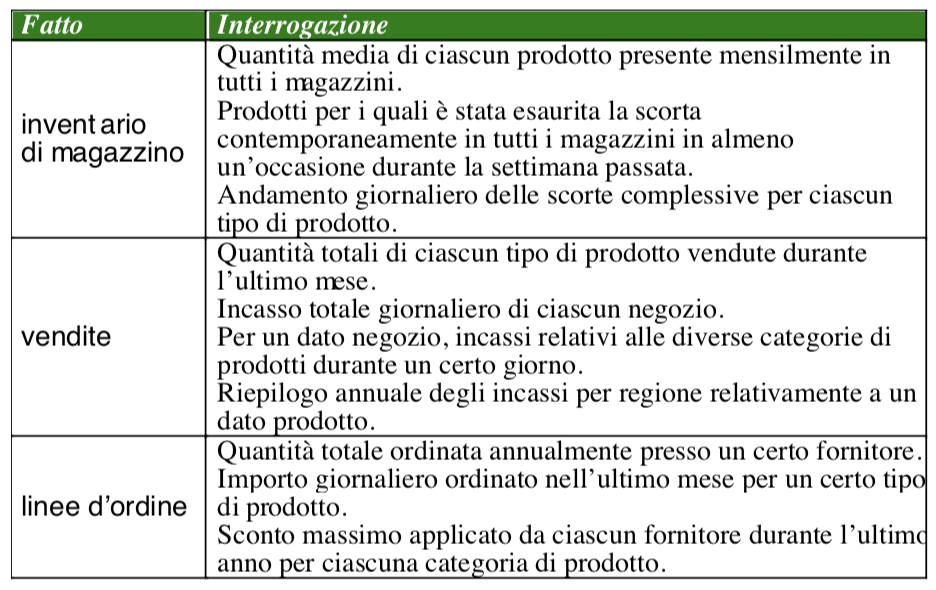
\includegraphics[scale=0.38]{Preliminare}
	\end{figure}
\end{multicols}

\noindent
Altri requisiti sono: vincoli di progettazione logica e fisica (spazio disponibile), progetto dell'alimentazione (periodicità dell'alimentazione), architettura del sistema di data warehousing (architettura da implementare, numero di livelli, presenza di data mart dipendenti o indipendenti, materializzazione del livello riconciliato), applicazioni per l'analisi dei dati (analisi delle tipologie di interrogazioni e dei rapporti analitici normalmente richiesti), piano di avviamento e piano di formazione.


\subsection*{Progettazione Concettuale}
\addcontentsline{toc}{subsection}{Progettazione Concettuale}
\MakeUppercase{è} universalmente riconosciuto che un DW si appoggia sul modello multidimensionale, ma non c'è accordo sulla metodologia di progetto concettuale (il modello entità/relazione non può essere usato per modellare i DW).
\\\\
Il \textit{\textbf{Dimensional Fact Model} (\textbf{DFM})} è un modello concettuale grafico per data mart pensato per: supportare il progetto concettuale, creare un ambiente su cui formulare in modo intuitivo le
interrogazioni dell’utente, permettere il dialogo tra progettista e utente finale per raffinare le specifiche dei requisiti, creare una piattaforma stabile da cui partire per il progetto logico (indipendentemente dal modello logico), restituire una documentazione espressiva e non ambigua.\\
La rappresentazione concettuale del \textit{DFM} consiste in un insieme di \textit{\textbf{schemi di fatto}}.\\
Gli \textbf{elementi di base} da modellare sono:
\begin{itemize}
	\item \textit{\textbf{fatti}}: modella un insieme di eventi che accadono nell’impresa (vendite, spedizioni, acquisti $\dots$). \MakeUppercase{è} essenziale che un fatto abbia aspetti dinamici, ovvero evolva nel tempo;
	\item \textit{\textbf{misure}}: proprietà numerica di un fatto e ne descrive un aspetto quantitativo per l’analisi (vendita misurata dall'incasso); uno \textbf{schema di fatto} si dice \textbf{vuoto} se non ha misure (il fatto registra solo il verificarsi di un evento).
	\item \textit{\textbf{dimensione}}: proprietà di un fatto e ne descrive una coordinata di analisi (per le vendite sono prodotto, negozio, data).
\end{itemize}
I \textbf{costrutti di base} del \textit{DFM} sono:
\begin{itemize}
	\item \textit{\textbf{attributi dimensionali}}: dimensioni ed eventuali altri attributi che le descrivono (un prodotto è descritto dal suo tipo, dalla categoria cui appartiene, dalla sua marca, dal reparto in cui è venduto);
	\item \textit{\textbf{gerarchia}}: albero direzionato i cui nodi sono attributi dimensionali e i cui archi modellano associazioni molti-a-uno tra coppie di attributi dimensionali. Racchiude una dimensione (alla radice dell’albero) e gli attributi dimensionali che la descrivono.
\end{itemize}
\begin{multicols}{2}
	\begin{figure}[H]
		\centering
		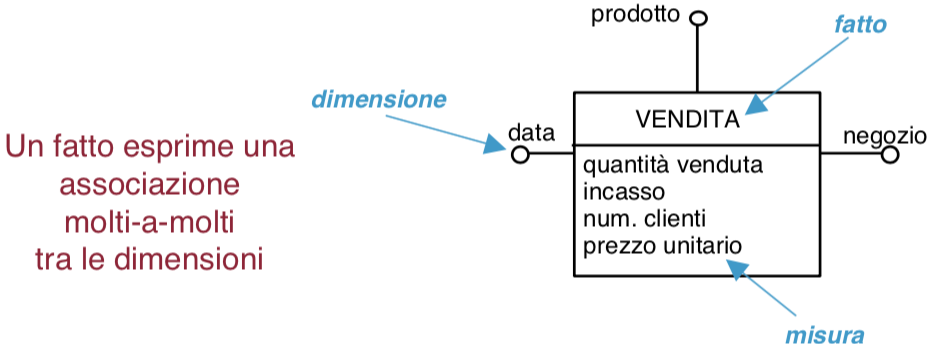
\includegraphics[scale=0.38]{DFM}
	\end{figure}
	\columnbreak
	\begin{figure}[H]
		\centering
		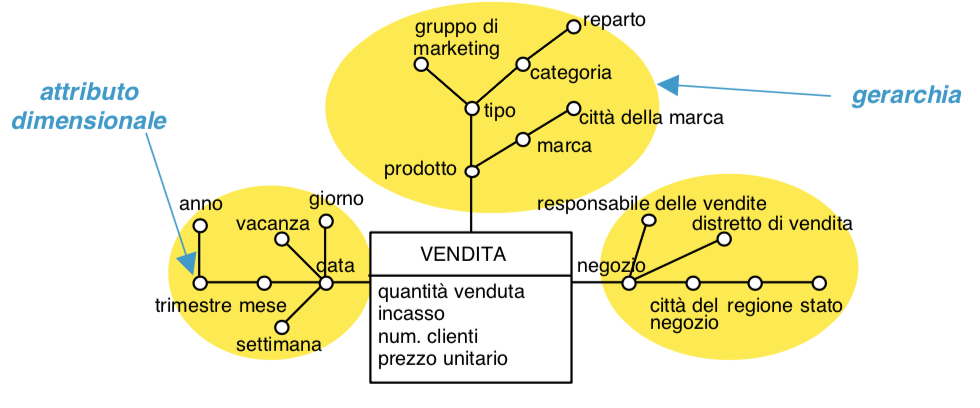
\includegraphics[scale=0.38]{DFM2}
	\end{figure}
\end{multicols}

\noindent
Le \textit{\textbf{Naming Conventions}} prevedono: attributi dimensionali con nomi diversi (nomi uguali devono essere differenziati con il nome di un attributo dimensionale che li precede nella gerarchia), i nomi degli attributi non dovrebbero riferirsi al fatto a cui appartengono (evitare \textit{shipped product} e \textit{shipment date}), attributi con stesso significato in schemi diversi devono avere stesso nome.
\\\\
\textbf{Costrutti avanzati}: un \textit{attributo descrittivo} contiene informazioni aggiuntive su un attributo dimensionale di una gerarchia. Non viene usato per l’aggregazione poiché ha valori continui e/o poiché deriva da un’associazione uno-a-uno (alcuni archi dello schema possono essere \textit{opzionali}).
\\\\
\textbf{Additività}: l'aggregazione richiede di definire un operatore adatto (SUM, AVG, MIN, MAX) per comporre i valori delle misure che caratterizzano gli eventi primari in valori da abbinare a ciascun evento secondario. Ci sono tre categorie di misure:
\begin{itemize}
	\item \textit{\textbf{Misure di Flusso}}: si riferiscono a un periodo, al cui termine vengono valutate in modo cumulativo (il numero di prodotti venduti in un giorno, l’incasso mensile, il numero di nati in un anno);
	\item \textit{\textbf{Misure di Livello}}: vengono valutate in particolari istanti di tempo (n° prodotti in inventario, n° abitanti di una città);
	\item \textit{\textbf{Misure Unitarie}}: vengono valutate in particolari istanti di tempo, ma sono espresse in termini relativi (prezzo unitario di un prodotto, percentuale di sconto, cambio di una valuta)
\end{itemize}
\noindent
Una misura è detta \textit{additiva} su una dimensione se i suoi valori possono essere aggregati lungo la corrispondente gerarchia tramite l’operatore di somma, altrimenti è \textit{non-additiva}. Una misura \textit{\textbf{non-additiva}} è \textit{non-aggregabile} se nessun operatore di aggregazione può essere usato su di essa.
\\\\
Ci sono due diversi approcci alla progettazione concettuale:
\begin{itemize}
	\item \textit{\textbf{basata sui requisiti}}: ricavare dalle interviste condotte presso l'utente, un'indicazione precisa sui fatti da rappresentare, le misure che li descrivono e le gerarchie attraverso cui aggregarli utilmente. Il problema del collegamento tra lo schema concettuale e le sorgenti operazionali viene affrontato in seguito;
	\item \textit{\textbf{basata sulle sorgenti}}: si può definire lo schema concettuale in funzione della struttura delle sorgenti, evitando il complesso compito di stabilire il legame con esse a posteriori. Inoltre, è possibile derivare uno schema concettuale dagli schemi operazionali in modo pressoché automatico.
\end{itemize}
La progettazione concettuale viene effettuata a partire dalla documentazione relativa al database riconciliato (schemi E/R, schemi relazionali, schemi XML $\dots$). I passi di progettazione consistono nella definizione dei fatti e per ogni passo: costruzione albero degli attributi, editing dell'albero, definizione delle dimensioni, definizione delle dimensioni, creazione dello schema di fatto.
\\\\
\textbf{Definizione dei Fatti}: entità o relazioni che rappresentano archivi frequentemente modificati (come VENDITA) possono definire \textit{fatti}; non è così per quelli che rappresentano archivi quasi-statici. Ogni fatto identificato diventa la radice di un nuovo schema.
\\\\
\textbf{Costruzione dell'Albero degli Attributi}: è un albero in cui ogni vertice corrisponde a un attributo dello schema sorgente, la radice corrisponde all'identificatore (chiave primaria), per ogni vertice $v$, l'attributo corrispondente determina tutti gli attributi corrispondenti ai discendenti di $v$. L’albero degli attributi può essere costruito in modo automatico applicando una procedura che naviga ricorsivamente le dipendenze espresse, nello schema sorgente, dagli identificatori e dalle associazioni a-uno.
\begin{multicols}{2}
	\begin{figure}[H]
		\centering
		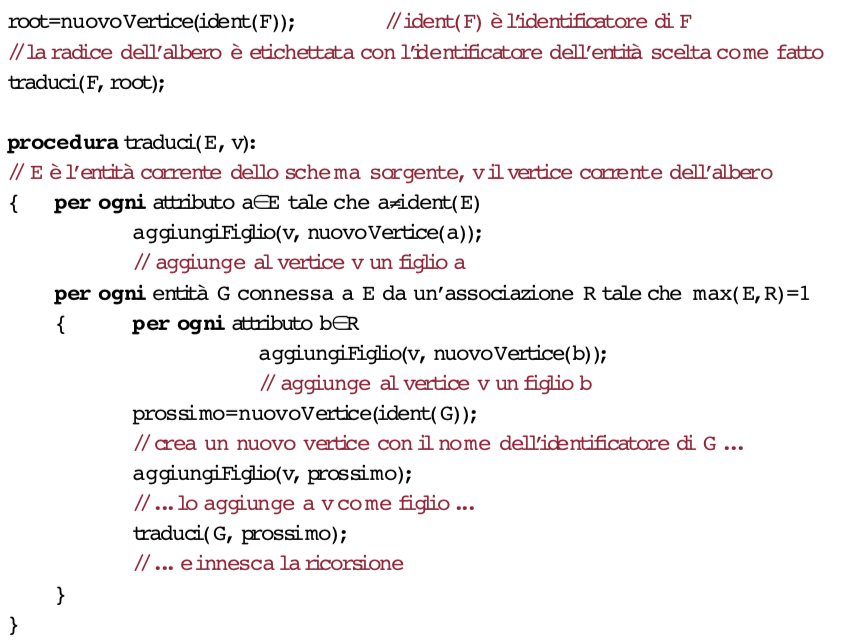
\includegraphics[scale=0.4]{Albero}
	\end{figure}
	\columnbreak
	\begin{figure}[H]
		\centering
		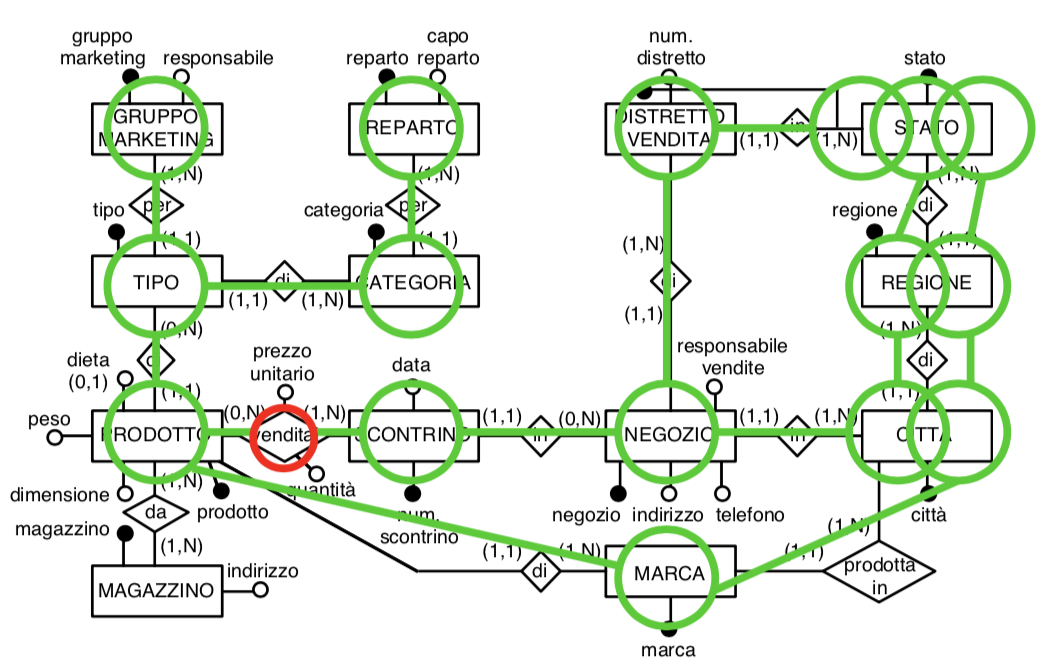
\includegraphics[scale=0.4]{Esempio}
	\end{figure}
\end{multicols}
\noindent
\textbf{Editing dell'Albero degli Attributi}: non tutti gli attributi dell’albero sono d’interesse per il data mart; quindi, l’albero può essere manipolato per eliminare i livelli di dettaglio non necessari.
\begin{multicols}{2}
	\noindent
	La \textit{potatura} di un vertice $v$ si effettua eliminando l’intero sottoalbero con radice in $v$. L’\textit{innesto} viene utilizzato quando, sebbene un vertice esprima un’informazione non interessante, è necessario mantenere nell’albero i suoi discendenti. L’innesto del vertice $v$, con padre $v'$, viene effettuato collegando tutti i figli di $v$ direttamente a $v'$ ed eliminando $v$. Quando un vertice opzionale viene innestato, tutti i suoi figli ereditano il trattino di opzionalità.
\columnbreak
	\begin{figure}[H]
		\centering
		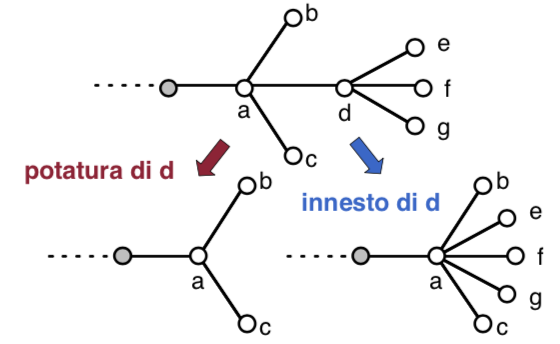
\includegraphics[scale=0.39]{Innesto}
	\end{figure}
\end{multicols}
\begin{multicols}{2}	
\noindent
Può anche essere necessario modificarne radicalmente la struttura sostituendo il padre di un certo nodo: ciò corrisponde ad aggiungere o eliminare una dipendenza.
\columnbreak
\begin{figure}[H]
	\centering
	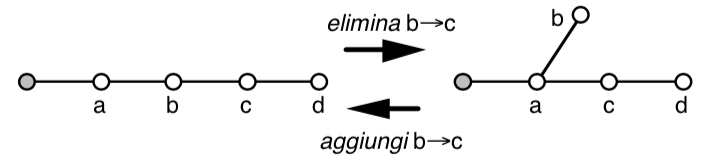
\includegraphics[scale=0.4]{Editing}
\end{figure}
\end{multicols}
\noindent
\textbf{Definizione delle Dimensioni}: devono essere scelte nell’albero degli attributi tra i vertici figli della radice; possono corrispondere ad attributi discreti o a intervalli di valori di attributi discreti o continui. La loro scelta definisce la granularità degli eventi primari. 
\begin{multicols}{2}
	\noindent
	Il tempo dovrebbe sempre essere una dimensione se:
	\begin{itemize}
		\item la sorgente è uno schema storico e il tempo è rappresentato esplicitamente come un attributo; se appare nell’albero degli attributi come figlio di un vertice diverso dalla radice, si può effettuare un innesto o eliminare una dipendenza per farlo diventare un figlio diretto della radice e quindi una dimensione.
		\item nelle sorgenti snapshot il tempo non è rappresentato; viene aggiunto manualmente allo schema di fatto.
	\end{itemize}
	\columnbreak
	\begin{figure}[H]
		\centering
		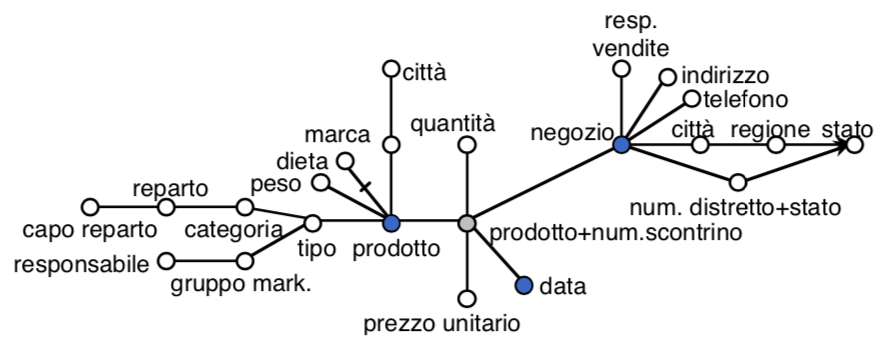
\includegraphics[scale=0.43]{Dimensioni}
	\end{figure}
\end{multicols}
\begin{multicols}{2}
	\noindent
	\textbf{Definizione delle Misure}: se tra le dimensioni compaiono tutti gli attributi che costituiscono un identificatore dell’entità fatto, allora le misure corrispondono ad attributi numerici che siano figli della radice dell’albero.\\\\
	In caso contrario le misure devono essere definite applicando, ad attributi numerici dell’albero, funzioni di aggregazione (SUM, MAX, MIN, AVG, COUNT) che operano su tutte le istanze corrispondenti a ciascun evento primario (un fatto può non avere misure; la sua granularità può differire da quella dello schema sorgente e si definiscono più misure che aggregano lo stesso attributo con operatori diversi).
	\columnbreak
	\begin{figure}[H]
		\centering
		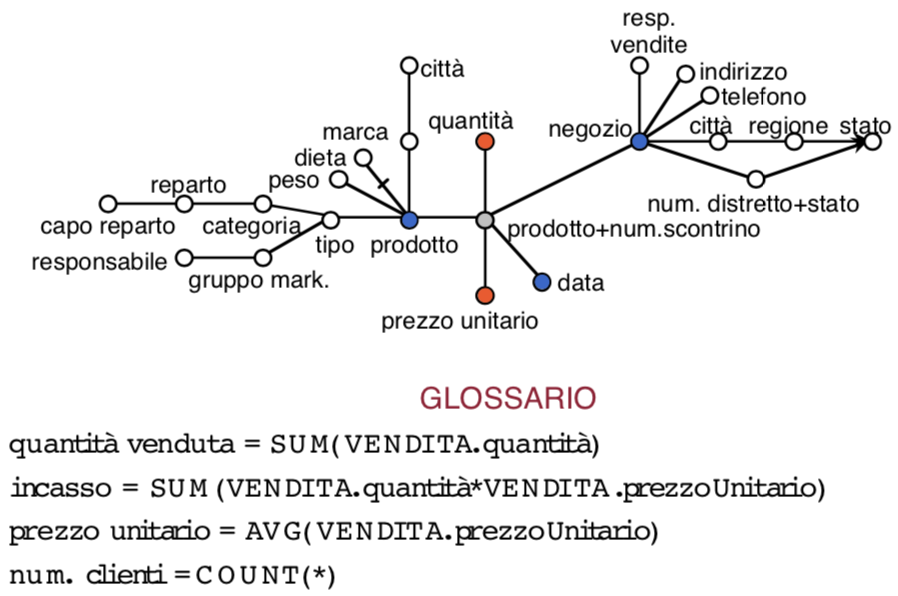
\includegraphics[scale=0.38]{Misure}
	\end{figure}
\end{multicols}
\noindent
\textbf{Creazione dello Schema di Fatto}: l’albero degli attributi si traduce in uno schema di fatto che include dimensioni e misure definite.
\begin{itemize}
	\item le gerarchie corrispondono ai sottoalberi dell’albero degli attributi con radice nelle diverse dimensioni;
	\item il nome del fatto corrisponde al nome dell’entità scelta come fatto;
	\item è possibile potare e innestare l’albero per eliminare dettagli inutili;
\end{itemize}
\begin{multicols}{2}
\begin{itemize}
	\item è possibile aggiungere attributi dimensionali definendo opportuni intervalli per attributi numerici (es. sulla dimensione tempo);
	\item gli attributi che non verranno usati per l’aggregazione possono essere contrassegnati come descrittivi; tra questi compariranno anche gli attributi determinati da associazioni uno-a-uno e privi di discendenti;
	\item attributi alfanumerici figli della radice ma non prescelti né come dimensioni né come misure, se la granularità degli eventi primari corrisponde a quella dell'entità verranno rappresentati come attributi descrittivi (altrimenti devono essere potati).
\end{itemize}
\columnbreak
\begin{figure}[H]
	\centering
	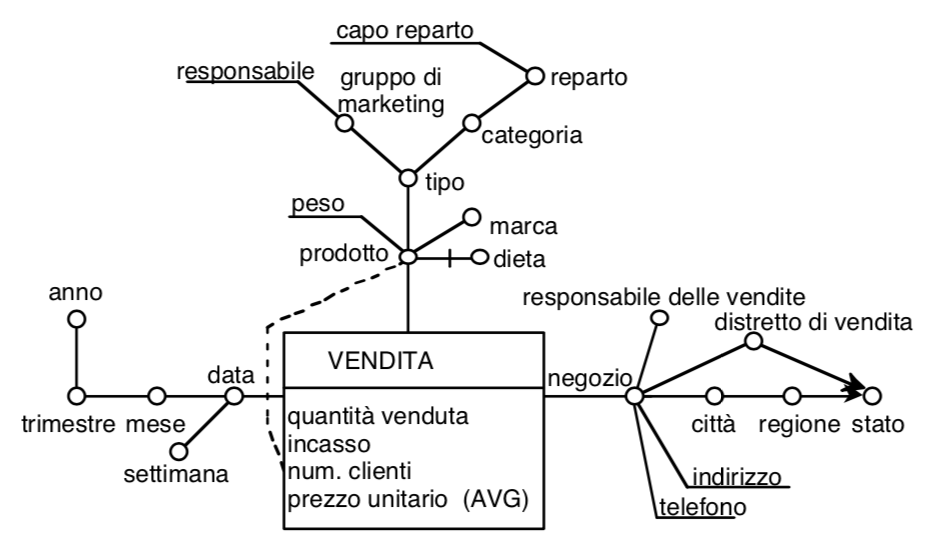
\includegraphics[scale=0.4]{Schema}
\end{figure}
\end{multicols}
\noindent
Eventuali attributi cross-dimensionali e archi multipli possono essere evidenziati in questa fase. Identificare questi attributi a partire dallo schema sorgente è complesso, poiché richiede di navigare anche le associazioni a-molti, per cui si preferisce definirli a partire dai requisiti utente per rappresentarli solo successivamente sullo schema di fatto. In questa fase devono anche essere identificate le eventuali non-additività e non-aggregabilità presenti nello schema, considerando tutte le accoppiate dimensione-misura.
\begin{figure}[H]
	\centering
	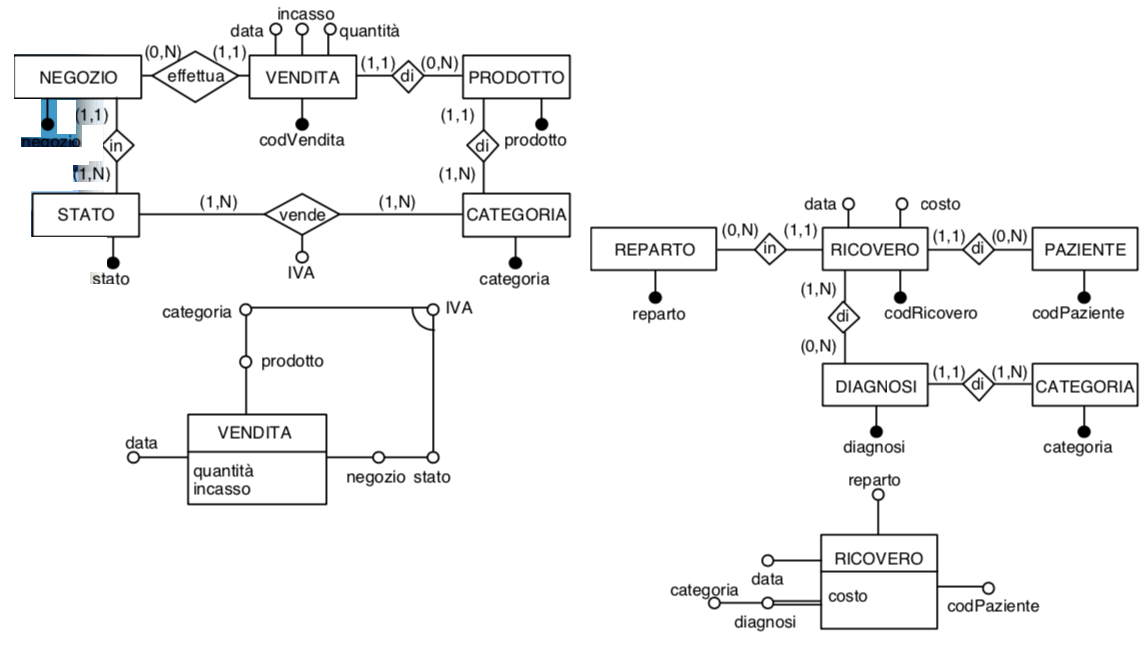
\includegraphics[scale=0.4]{Creazione}
\end{figure}


\subsection*{Carico di Lavoro e Volume Dati}
\addcontentsline{toc}{subsection}{Carico di Lavoro e Volume Dati}
È necessario identificare in fase di progettazione un carico di lavoro di riferimento (reportistica, standard, colloqui con gli utenti). Le interrogazioni \textit{OLAP} sono facilmente caratterizzabili: pattern di aggregazione, misure richieste, clausole di selezione.
\\
\textit{\textbf{Dinamicità del Carico di Lavoro}}: il carico di lavoro preliminare non è sufficiente per ottimizzare le prestazioni del sistema (l'interesse degli utenti cambia nel tempo e il numero di interrogazioni aumenta al crescere della confidenza degli utenti con il sistema). Per ottimizzare la struttura logica del data mart serve una fase di tuning attuabile solo dopo che il sistema è stato messo in funzione.
\\\\
\textit{\textbf{Il Volume di Dati}}: consiste nelle informazioni necessarie a determinare/stimare la dimensione del data mart (numero di valori distinti degli attributi nelle gerarchie, lunghezza degli attributi, numero di eventi di ogni fatto). È utilizzato sia durante la progettazione logica sia durante la progettazione fisica per determinare: dimensione delle tabelle, dimensione degli indici, costi di accesso. La bontà delle stime è spesso compromessa a causa del problema della sparsità.
\\\\
\textit{\textbf{Il Problema della Sparsità}}: nel modello multidimensionale, a un insieme di coordinate corrisponde un possibile evento anche se questo non è realmente avvenuto (il n° di eventi accaduti è molto inferiore a quelli possibili). Tenere traccia degli eventi non accaduti comporta uno spreco di risorse e riduce le prestazioni del sistema: \textit{ROLAP} (memorizza solo gli eventi accaduti), \textit{MOLAP} (richiede tecniche complesse per ridurre al minimo lo spazio necessario a tenere traccia degli eventi non accaduti).\\
La sparsità dei dati compromette le stime sulla cardinalità dei dati aggregati.\\
La sparsità si riduce all’aumentare del livello di aggregazione dei dati.


\section*{Progettazione Logica}
\addcontentsline{toc}{section}{Progettazione Logica}
La modellazione concettuale è indipendente dal modello logico, non è così per i temi legati alla modellazione logica. La struttura multidimensionale dei dati può essere rappresentata utilizzando due distinti modelli logici:
\begin{itemize}
	\item \textit{\textbf{MOLAP} (Multidimensional On-Line Analytical Processing)}: memorizzano i dati utilizzando strutture multidimensionali (es. vettori multidimensionali);
	\item \textit{\textbf{ROLAP} (Relational On-Line Analytical Processing)}: utilizza modello relazionale per rappresentare i dati multidimensionali.
\end{itemize}

\subsection*{Sistemi MOLAP}
\addcontentsline{toc}{subsection}{Sistemi MOLAP}
L'utilizzo di soluzioni \textit{MOLAP}:
\begin{itemize}
	\item può fornire ottime prestazioni poiché le operazioni non devono essere “simulate” mediante complesse istruzioni SQL; 
	\item pone il problema della \textit{sparsità}: in media solo il $20\%$ delle celle dei cubi contiene effettivamente informazioni, mentre le restanti celle corrispondono a fatti non accaduti;
	\item è frenato dalla mancanza di strutture dati standard: i diversi produttori di software utilizzano strutture proprietarie che li rendono difficilmente sostituibili e accessibili mediante strumenti di terze parti;
	\item progettisti e sistemisti non vogliono rinunciare alla loro lunga esperienza sui sistemi relazionali.
\end{itemize}
Le tecniche di \textit{\textbf{gestione della sparsità}} sono basate sui seguenti principi:
\begin{itemize}
	\item \textit{suddivisione delle dimensioni}: consiste nel partizionare un cubo n-dimensionale in più sottocubi n-dimensionali (\textit{chunk}). I singoli chunk potranno essere caricati più agevolmente in memoria e saranno gestiti in modo differente a seconda che siano \textit{densi} (la maggior parte delle celle contiene informazioni) oppure \textit{sparsi} (la maggior parte non contiene informazioni).
	\item \textit{compressione dei chunk sparsi}: essi vengono rappresentati in forma compressa al fine di evitare lo spreco di spazio dovuto alla rappresentazione di celle che non contengono informazioni. Una struttura dati comunemente usata prevede un indice che riporti il solo offset delle celle che effettivamente contengono informazioni.
\end{itemize}

\subsection*{Sistemi ROLAP: Schema a Stella}
\addcontentsline{toc}{subsection}{Sistemi ROLAP: Schema a Stella}
La modellazione multidimensionale su sistemi relazionali è basata sullo schema a stella (\textit{star schema}) e sulle sue varianti.\\
Uno \textbf{schema a stella} è composto da:
\begin{itemize}
	\item un insieme di relazioni $DT_1, \dots , DT_n$, chiamate \textit{dimension table}, ciascuna corrispondente a una dimensione. Ogni $DT_i$ è caratterizzata da una chiave primaria $d_i$ e da attributi che descrivono le dimensioni di analisi a diversi livelli di aggregazione;
	\item una relazione $FT$, chiamata \textit{fact table}, che importa le chiavi di tutte le \textit{dimension table}. La chiave primaria di $FT$ è data dall’insieme delle chiavi esterne dalle \textit{dimension table}, $d_1, \dots , d_n$; $FT$ contiene inoltre un attributo per ogni misura.
\end{itemize}
Non si hanno problemi di \textit{sparsità} in quanto vengono memorizzate soltanto le tuple corrispondenti a punti dello spazio multi-dimensionale per cui esistono eventi
\begin{multicols}{2}
\begin{figure}[H]
	\centering
	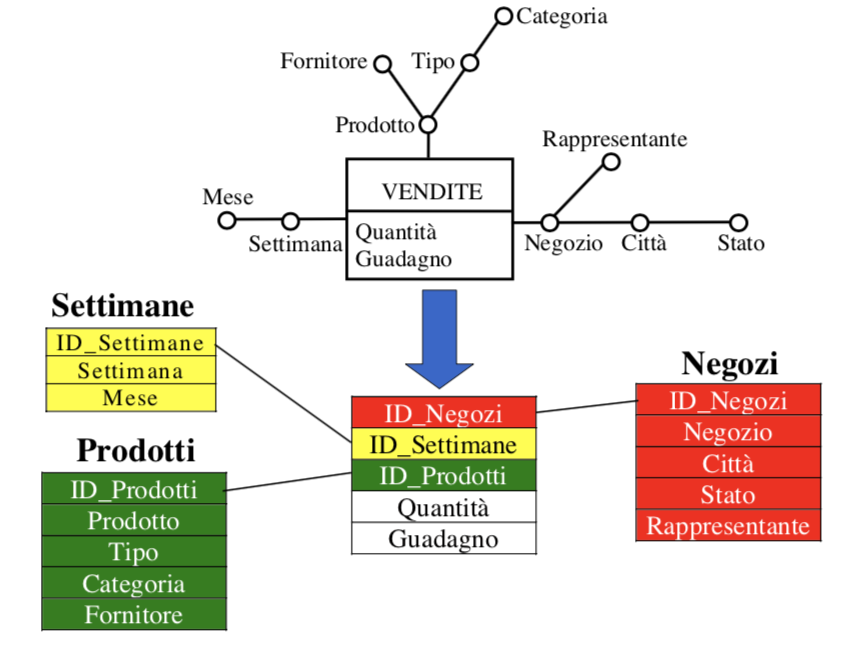
\includegraphics[scale=0.38]{Stella}
\end{figure}
\columnbreak
\begin{figure}[H]
	\centering
	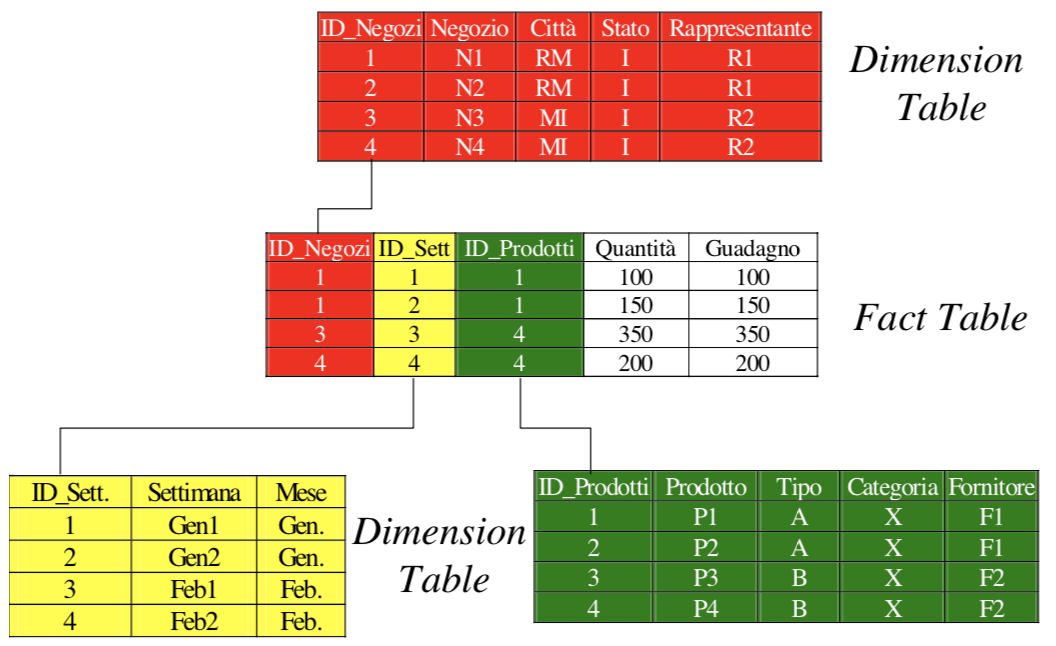
\includegraphics[scale=0.38]{Stella2}
\end{figure}
\end{multicols}
\noindent
Le \textit{Dimension Table} sono completamente denormalizzate (es. Prodotto $\rightarrow$ Tipo); è sufficiente un join per recuperare tutti i dati relativi a una dimensione. La denormalizzazione introduce una forte ridondanza nei
dati.\\
La \textit{Fact Table} contiene tuple relative a diversi livelli di aggregazione (l'elevata dimensione incide sui tempi di accesso ai dati).

\subsection*{Snowflake Schema}
\addcontentsline{toc}{subsection}{Snowflake Schema}
Lo \textit{\textbf{schema a fiocco di neve}} riduce la denormalizzazione delle \textit{dimension table} $DT_i$ degli schemi a stella eliminando alcune delle dipendenze transitive che le caratterizzano. Le \textit{dimension table} $DT_{i,j}$ di questo schema sono caratterizzate da:
\begin{itemize}
	\item una chiave primaria $d_{i,j}$;
	\item il sottoinsieme degli attributi di $DT_i$ che dipendono funzionalmente da $d_{i,j}$;
	\item zero o più chiavi esterne importate da altre $DT_{i,k}$ necessarie a garantire la ricostruibilità del contenuto informativo di $DT_i$.
\end{itemize}
Denominiamo \textbf{primarie} le \textit{dimension table} le cui chiavi sono importate nella \textit{fact table}, \textbf{secondarie} le rimanenti.\\
Lo spazio richiesto per la memorizzazione dei dati si riduce grazie alla normalizzazione. È necessario inserire nuove chiavi surrogate per determinare le corrispondenze tra \textit{dimension table} primarie e secondarie.\\\\
L’esecuzione di interrogazioni che coinvolgono solo gli attributi contenuti nella \textit{fact table} e nelle \textit{dimension table} primarie è avvantaggiata. Il tempo di esecuzione delle interrogazioni che coinvolgono attributi delle \textit{dimension table} secondarie aumenta.\\
Lo \textit{snowflake schema} è particolarmente utile in presenza di dati aggregati.
\begin{multicols}{2}
\begin{figure}[H]
	\centering
	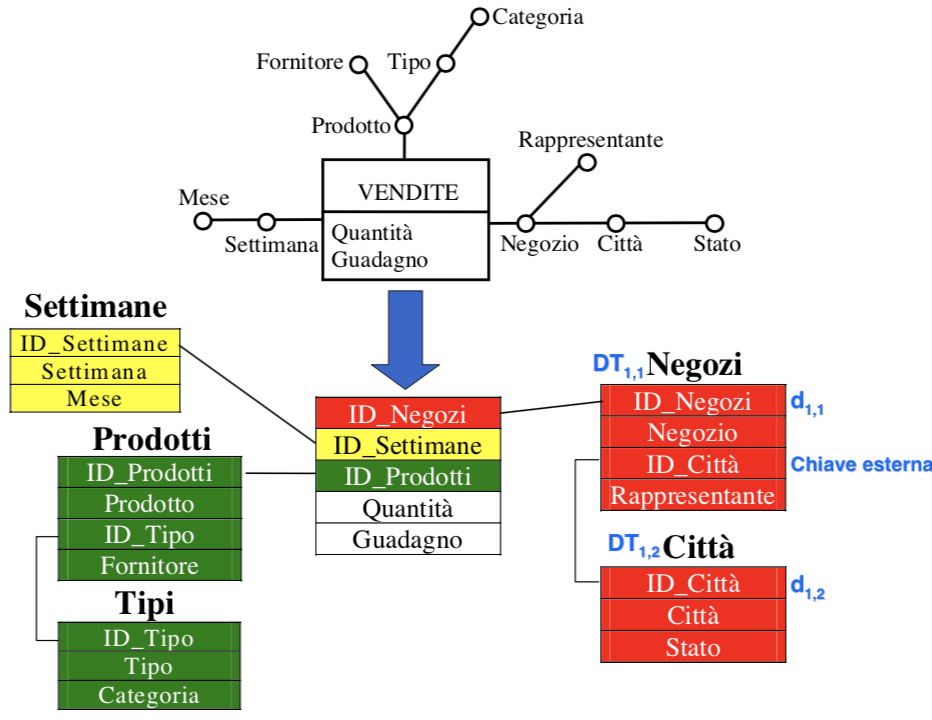
\includegraphics[scale=0.38]{Snowflake}
\end{figure}
\columnbreak
\begin{figure}[H]
	\centering
	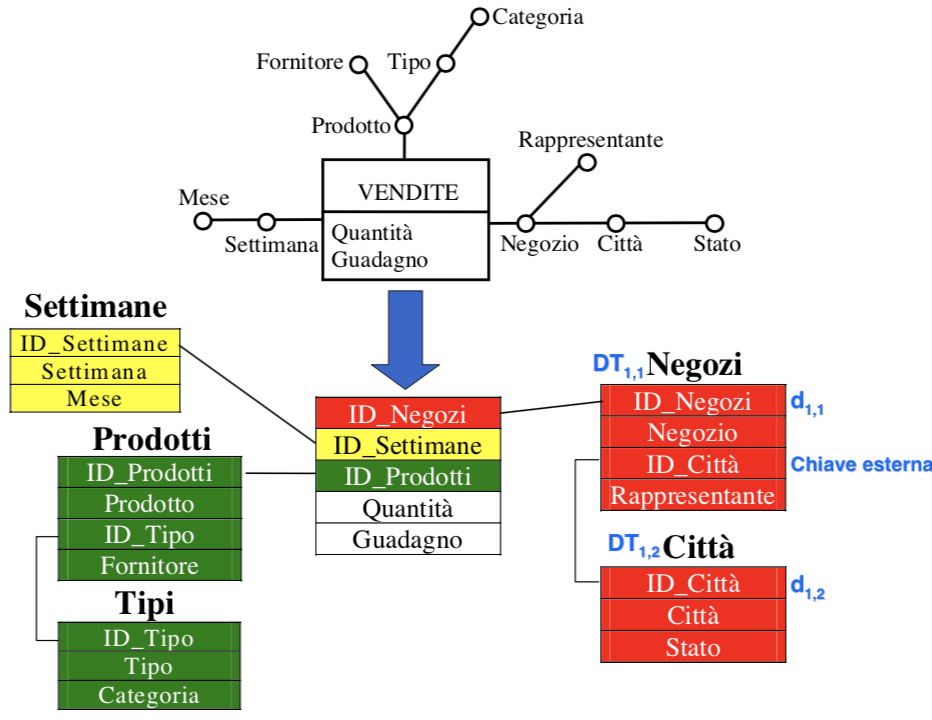
\includegraphics[scale=0.38]{Snowflake}
\end{figure}
\end{multicols}
\begin{multicols}{2}
	\noindent
	\textit{\textbf{Normalizzazione con lo Snowflake Schema}}: le caratteristiche degli schemi a stella richiedono particolare attenzione affinché nella nuova relazione sia spostato il corretto insieme di attributi. La presenza di più dipendenze funzionali transitive in cascata fa sì che, affinché la decomposizione sia efficace, tutti gli attributi che dipendono dall’attributo che ha determinato lo snowflaking siano posti nella nuova relazione.
	\columnbreak
	\begin{figure}[H]
		\centering
		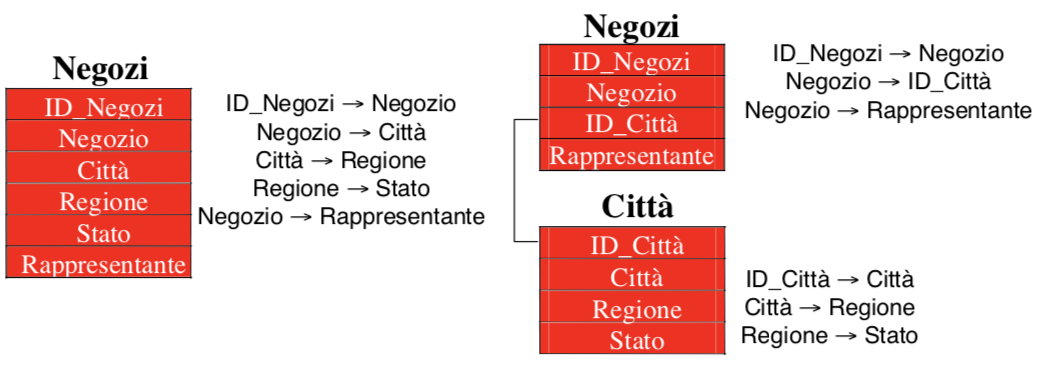
\includegraphics[scale=0.38]{Normalizzazione}
	\end{figure}
\end{multicols}



\end{document}